% !TeX spellcheck = en-US
% LTeX: language=en-US
% !TeX encoding = utf8
% !TeX program = lualatex
% !TeX TXS-program:compile = txs:///lualatex/[--shell-escape]
% !BIB program = biber
% -*- coding:utf-8 mod:LaTeX -*-

\RequirePackage{kvoptions-patch}
\documentclass[
  numbers=noenddot,
  english,
  a4paper,
  twoside,
  bibliography=totoc,
  headsepline,
  cleardoublepage=empty,
  parskip=half,
  draft=false
]{scrbook}

\usepackage[
  a4paper,
  left=2.5cm,
  right=2.5cm,
  top=3cm,
  bottom=3cm
]{geometry}

\usepackage{scrlayer-scrpage}

\usepackage{iftex}
\usepackage{ifplatform}
\usepackage{upquote}

\usepackage[ngerman,main=english]{babel}
\addto\extrasenglish{\languageshorthands{ngerman}\useshorthands{"}}

\usepackage[hyphens]{url}

\makeatletter
\g@addto@macro{\UrlBreaks}{\UrlOrds}
\makeatother

\usepackage[
  centertags,
  sumlimits,
  intlimits,
  namelimits,
  fleqn,
]{amsmath}
\SetMathAlphabet{\mathcal}{normal}{OMS}{amsa}{m}{n}

\usepackage[fixamsmath,disallowspaces]{mathtools}
\usepackage{fixmath}

\usepackage[amsmath,hyperref]{ntheorem}
\theorempreskipamount 2ex plus1ex minus0.5ex
\theorempostskipamount 2ex plus1ex minus0.5ex
\theoremstyle{break}
\newtheorem{definition}{Definition}[chapter]

\ifluatex
  \usepackage[no-math]{fontspec}
  \usepackage{unicode-math}
  \setmainfont{texgyretermes}[
    Extension = .otf,
    UprightFont = *-regular,
    BoldFont = *-bold,
    ItalicFont = *-italic,
    BoldItalicFont = *-bolditalic,
    Ligatures=TeX
  ]
  \setsansfont[Scale=.9]{TeX Gyre Heros Regular}
  \ifwindows
    \setmonofont[StylisticSet={1,3},Scale=.9]{Inconsolata}
  \else
    \setmonofont[StylisticSet={1,3},Scale=.9]{Inconsolatazi4}
  \fi
  \usepackage{selnolig}
\else
  \RequirePackage{newtxtext}
  \RequirePackage{newtxmath}
  \RequirePackage[zerostyle=b,scaled=.9]{newtxtt}
  \usepackage[T1]{fontenc}
\fi

\usepackage{setspace}

\usepackage{pifont}
\newcommand{\dingcheck}{\ding{51}}
\newcommand{\dingcross}{\ding{55}}

\automark[section]{chapter}
\setkomafont{pageheadfoot}{\normalfont\sffamily}
\setkomafont{pagenumber}{\normalfont\sffamily}

\ihead[]{}
\chead[]{}
\ohead[]{\headmark}
\cfoot[]{}
\ofoot[\usekomafont{pagenumber}\thepage]{\usekomafont{pagenumber}\thepage}
\ifoot[]{}

\usepackage[
  babel=true,
  expansion=alltext,
  protrusion=alltext-nott,
  final
]{microtype}

\DisableLigatures{encoding = T1, family = tt* }

\usepackage{graphicx}
\graphicspath{ {figures/} }

\usepackage{pdfpages}
\usepackage{diagbox}

\usepackage[dvipsnames, table]{xcolor}
\usepackage[newfloat]{minted}

\setminted{
  numbersep=5pt,
  xleftmargin=12pt,
  breakafter=-/,
  breakbefore=\\
}

\usemintedstyle{friendly_grayscale}

\usepackage[labelfont=bf,font=small,skip=4pt]{caption}
\SetupFloatingEnvironment{listing}{name=List.,within=none}

\newcommand{\labelline}[1]{\label[line]{#1}\hypertarget{#1}{}}
\newcommand{\refline}[1]{\hyperlink{#1}{\FancyVerbLineautorefname~\ref*{#1}}}

\usepackage[autostyle=true]{csquotes}
\defineshorthand{"`}{\openautoquote}
\defineshorthand{"'}{\closeautoquote}

\usepackage{booktabs}
\usepackage{paralist}

\usepackage[
  backend       = biber,
  sortcites     = true,
  sorting       = none,
  bibstyle      = numeric,
  citestyle     = numeric-comp,
  giveninits    = true,
  useprefix     = false,
  minnames      = 1,
  maxbibnames   = 99,
  maxcitenames  = 2,
  natbib        = true,
  eprint        = true,
  url           = true,
  doi           = true,
  isbn          = true,
  backref       = true]{biblatex}

\setcounter{biburllcpenalty}{7000}
\setcounter{biburlucpenalty}{8000}

\bibliography{bibliography}

\makeatletter
\AtBeginDocument{\toggletrue{blx@useprefix}}
\AtBeginBibliography{\togglefalse{blx@useprefix}}
\makeatother

\renewrobustcmd*{\bibinitdelim}{\,}
\renewcommand*\bibnamedelimc{\addnbspace}
\renewcommand*\bibnamedelimd{\addnbspace}

\AtBeginBibliography{%
  \renewcommand*{\finalnamedelim}{\addcomma\space}%
}

\DeclareCiteCommand{\citeauthor}
{
  \boolfalse{citetracker}%
  \boolfalse{pagetracker}%
  \usebibmacro{prenote}
}
{
  \ifciteindex
  {\indexnames{labelname}}
  {}%
  \printtext[bibhyperref]{\printnames{labelname}}
}
{\multicitedelim}
{\usebibmacro{postnote}}

\usepackage{multirow}
\usepackage{dcolumn}

\usepackage[
  bottom,
  stable,
  ragged,
  multiple,
]{footmisc}

\counterwithout{footnote}{chapter}
\interfootnotelinepenalty=10000

\usepackage{stfloats}
\fnbelowfloat

\usepackage{pdfcomment}

\newcommand{\textcomment}[2]{\colorbox{yellow!60}{#1}\pdfcomment[color={0.234 0.867 0.211},hoffset=-6pt,voffset=10pt,opacity=0.5]{#2}}
\newcommand{\sidecomment}[1]{\pdfcomment[color={0.045 0.278 0.643},voffset=4pt,icon=Note]{#1}}
\newcommand{\todo}[1]{TODO!\sidecomment{#1}}
\newcommand{\change}[2]{{\color{red}#2}\pdfcomment[color={0.234 0.867 0.211},voffset=8pt,opacity=0.5]{#1}}

\makeatletter
\@ifundefined{missingfigure}{\newcommand{\missingfigure}[1]{\framebox[\linewidth]{\parbox{\linewidth}{\centering\vspace{2cm}\textit{[Figure placeholder: #1]}\vspace{2cm}}}}}{}
\@ifundefined{textcomment}{\newcommand{\textcomment}[2]{#1 \todo{#2}}}{}
\@ifundefined{sidecomment}{\newcommand{\sidecomment}[1]{\marginpar{#1}}}{}
\@ifundefined{todo}{\newcommand{\todo}[1]{\sidecomment{#1}}}{}
\@ifundefined{TODO}{\newcommand{\TODO}[1]{\todo{#1}}}{}
\@ifundefined{todofix}{\newcommand{\todofix}[1]{\todo{#1}}}{}
\@ifundefined{change}{\newcommand{\change}[2]{#1 $\rightarrow$ #2}}{}
\makeatother

\newcommand{\textmarker}[1]{{\color{red} #1}\xspace}
\newcommand{\modified}[1]{{\color{blue!60!black} #1}\xspace}

\usepackage[group-minimum-digits=4,per-mode=fraction]{siunitx}

\usepackage{varioref}

\usepackage{hyperref}
\hypersetup{
  hidelinks,
  colorlinks=true,
  raiselinks=true,
  allcolors=black,
  pdfstartview=Fit,
  breaklinks=true,
  hypertexnames=false,
}

\usepackage[all]{hypcap}
\usepackage{pdflscape}
\usepackage[caption=false,font=footnotesize]{subfig}
\usepackage{mindflow}

\usepackage[chapter]{algorithm}
\usepackage{algpseudocodex}

\floatname{algorithm}{Algorithm}
\renewcommand{\listalgorithmname}{List of Algorithms}

\newcommand{\commentchar}{\ensuremath{/\mkern-4mu/}}
\algrenewcommand{\algorithmiccomment}[1]{\hfill $\commentchar$ #1}

\usepackage[capitalise,nameinlink,noabbrev]{cleveref}

\crefname{listing}{Listing}{Listings}
\Crefname{listing}{Listing}{Listings}

\newcommand{\llabel}[1]{\label[line]{#1}\hypertarget{#1}{}}
\newcommand{\lref}[1]{\hyperlink{#1}{\FancyVerbLineautorefname~\ref*{#1}}}

\usepackage{lipsum}
\usepackage[math]{blindtext}
\usepackage{mwe}
\usepackage[realmainfile]{currfile}
\usepackage{tcolorbox}
\tcbuselibrary{minted}

\DeclareFontFamily{U}{MnSymbolC}{}
\DeclareSymbolFont{MnSyC}{U}{MnSymbolC}{m}{n}
\DeclareFontShape{U}{MnSymbolC}{m}{n}{
  <-6>    MnSymbolC5
  <6-7>   MnSymbolC6
  <7-8>   MnSymbolC7
  <8-9>   MnSymbolC8
  <9-10>  MnSymbolC9
  <10-12> MnSymbolC10
  <12->   MnSymbolC12%
}{}
\DeclareMathSymbol{\powerset}{\mathord}{MnSyC}{180}

\usepackage[
  translate=babel,
  abbreviations,
  nomain,
  stylemods=longbooktabs,
  automake
]{glossaries-extra}
\setglossarystyle{long3col-booktabs}

\makeglossaries

% Abbreviations / Acronyms used in the preCICE AI thesis
% Used with the glossaries-extra package

\newacronym{mcp}{MCP}{Model Context Protocol}
\newacronym{llm}{LLM}{Large Language Model}
\newacronym{rag}{RAG}{Retrieval-Augmented Generation}
\newacronym{cli}{CLI}{Command-Line Interface}
\newacronym{api}{API}{Application Programming Interface}
\newacronym{xml}{XML}{Extensible Markup Language}
\newacronym{json}{JSON}{JavaScript Object Notation}
\newacronym{fsi}{FSI}{Fluid-Structure Interaction}
\newacronym{cht}{CHT}{Conjugate Heat Transfer}
\newacronym{rbf}{RBF}{Radial Basis Function}
\newacronym{rpc}{RPC}{Remote Procedure Call}
\newacronym{sdk}{SDK}{Software Development Kit}
\newacronym{gpu}{GPU}{Graphics Processing Unit}
\newacronym{cpu}{CPU}{Central Processing Unit}
\newacronym{hpc}{HPC}{High-Performance Computing}
\newacronym{ui}{UI}{User Interface}
\newacronym{qa}{Q\&A}{Question and Answer}
\newacronym{ide}{IDE}{Integrated Development Environment}
\newacronym{nlp}{NLP}{Natural Language Processing}
\newacronym{bm25}{BM25}{Best Match 25}
\newacronym{url}{URL}{Uniform Resource Locator}
\newacronym{http}{HTTP}{Hypertext Transfer Protocol}
\newacronym{io}{I/O}{Input/Output}

\usepackage{xspace}
\makeatletter
\xspaceaddexceptions{\grqq \grq \csq@qclose@i \} }
\makeatother

\newcommand{\eg}{e.g.,\ }
\newcommand{\ie}{i.e.,\ }

\makeatletter
\newcommand{\hydash}{\penalty\@M-\hskip\z@skip}
\makeatother

% correct bad hyphenation here
\hyphenation{
  op-tical net-works semi-conduc-tor
  AROMA TOSCA BPMN OASIS OMG DMTF IT DevOps preCICE MCP
}

% Custom commands for the preCICE AI thesis

% Shorthand for preCICE (consistent formatting)
\newcommand{\precice}{preCICE\xspace}

% Shorthand for preCICE AI
\newcommand{\preciceai}{preCICE AI\xspace}

% Shorthand for the config file name
\newcommand{\preciceconfig}{\texttt{precice-config.xml}\xspace}

% Shorthand for CLAUDE.md
\newcommand{\claudemd}{\texttt{CLAUDE.md}\xspace}

% Tool name formatting
\newcommand{\tool}[1]{\texttt{#1}}

\usepackage[
  title={preCICE AI},
  author={Vaibhav Dange},
  type=master,
  institute=ipvs,
  course={Computer Science},
  examiner={Prof.\ Dr.\ Benjamin Uekermann},
  supervisor={Felix Neubauer},
  startdate={April 20, 2026},
  enddate={October 20, 2026},
  language=english
]{scientific-thesis-cover}

\ifpdftex
  \input{glyphtounicode}
  \pdfgentounicode=1
\fi

\usepackage{calc}

\newcommand*\Descriptionlabel[1]{%
  \raisebox{0pt}[1ex][0pt]{
    \makebox[\labelwidth][1]{
      \parbox[t]{\labelwidth}{
        \hspace{0pt}\textbf{#1:}}}}
}

\newcommand*\Descriptionlabelx[1]{%
  \parbox[t]{\textwidth}{
    \textbf{#1}\\\mbox{}}
}

\newenvironment{Description}{
  \begin{list}{}{
      \let\makelabel\Descriptionlabelx
      \setlength\labelwidth{1em}
      \setlength\leftmargin{\labelwidth+\labelsep}
    }
    }
    {
  \end{list}
}

\usepackage[inline]{enumitem}
\setlist{partopsep=0pt,itemsep=1pt}

\usepackage{xifthen}
\definecolor{quotemark}{gray}{0.7}

\newenvironment{fquote}[1][]{%
  \newcommand{\fqauthor}{\relax}
  \ifthenelse{\isempty{#1}}
  {}%
  {\renewcommand{\fqauthor}{\hfill\textsc{--- #1}}}
  \vspace{1em}
  \begin{list}{}{%
      \setlength{\leftmargin}{0.2\textwidth}
      \setlength{\rightmargin}{0.2\textwidth}
    }
    \item[]%
          \begin{picture}(0,0)(0,0)
            \put(-15,-5){\makebox(0,0){%
                \scalebox{4.5}{\textcolor{quotemark}{\bfseries``}}}%
            }
          \end{picture}\em\ignorespaces%
          }{%
          \newline%
          \makebox[0pt][l]{\hspace{0.6\textwidth}%
            \begin{picture}(0,0)(0,0)
              \put(15,10){\makebox(0,0){%
                  \scalebox{4.5}{\textcolor{quotemark}{\rmfamily\bfseries''}}}%
              }
            \end{picture}}%
          \fqauthor
  \end{list}
}

\usepackage{scrhack}


%%% ============================================================
\begin{document}
%%% ============================================================

\raggedbottom
\pagenumbering{arabic}
\Titelblatt

\pagestyle{plain.scrheadings}
\renewcommand*{\chapterpagestyle}{plain.scrheadings}

% ---------------------------------------------------------------
\section*{Abstract}
% ---------------------------------------------------------------

Multiphysics simulation software such as preCICE is a powerful enabler of partitioned coupled
simulations, yet its configuration complexity and steep learning curve present a considerable
barrier to new and occasional users.
This thesis investigates how an intelligent, context-aware assistant called \preciceai can lower
this barrier by integrating natural-language interaction directly into the local preCICE
simulation environment.

A gap exists between the capabilities of modern large language models and the practical usability
of simulation toolchains.
General-purpose assistants lack grounded access to local project state, configuration files, and
runtime logs, and are therefore unable to provide actionable, context-specific guidance.
Prior work on integrating language-model assistants into software systems has not addressed the
full local-tool integration challenge posed by scientific simulation frameworks, and no published
system covers the complete preCICE workflow from project setup to log-based diagnosis.

To address this gap, two complementary prototypes were designed and implemented.
The first is a preCICE-focused \gls{mcp} server that exposes project discovery, configuration
inspection, log analysis, a dual lexical-and-semantic knowledge base built from the preCICE
documentation, forum, and issue tracker, and a wrapper around the official \texttt{precice-cli},
to any \gls{mcp}-compatible client such as Claude Code, Codex, or Cursor.
The second is a self-contained agentic client built with LangGraph that runs a ReAct-style
tool-calling loop against a locally hosted browser interface, combines a purpose-built retrieval
pipeline with the same class of project, configuration, and log tools, and can in turn drive the
\gls{mcp} server as a subprocess.
Both prototypes share the goal of grounding the language model in the user's actual project state
rather than relying on its training data alone.

The two prototypes are evaluated through functional testing of the exposed tools and through a
scenario-based comparison spanning simulation setup, configuration error detection, and log
analysis, contrasting their usability, response accuracy, local integration, development
complexity, and extensibility against each other and against an ungrounded baseline.
Accuracy is assessed across two knowledge-base retrieval modes, several language models of
differing capability, and question sets of increasing difficulty, using a combination of
similarity-based scoring for narrowly defined questions and manual qualitative assessment for
open-ended ones.

The \gls{mcp}-based prototype exposes preCICE's local toolchain to a language-model assistant with
modest setup overhead, and early demonstrations indicate measurable improvements on preCICE-related
tasks compared with an assistant that has no access to the local project or to domain-specific
retrieval.
These results suggest that grounded, tool-integrated language-model assistants can meaningfully
narrow the usability gap in scientific simulation software, and point toward an architecture that
generalises to other simulation frameworks beyond preCICE.

\microtypesetup{protrusion=false}
\tableofcontents
\listoffigures
\listoftables
\listoflistings

\glsaddall
\printglossary[type=\acronymtype,title={Abbreviations}]

\microtypesetup{protrusion=true}

\renewcommand*{\chapterpagestyle}{scrplain}
\pagestyle{scrheadings}


%%% ===============================================================
\chapter{Introduction}\label{sec:introduction}
%%% ===============================================================

Multiphysics simulations are an indispensable tool across modern engineering and science,
enabling the study of coupled physical phenomena that cannot be captured by single-physics
models alone.
Setting up and operating such simulations requires integrating multiple solvers, managing data
exchange between them, and carefully configuring coupling parameters which is a process that demands
deep expertise and considerable time even from experienced practitioners.

preCICE is a widely adopted open-source coupling library that manages precisely this
complexity: it handles data mapping, communication, and synchronization between independent
solver codes \cite{chourdakis2022precice}.
However, the very breadth of its capabilities, which is configuration files, command-line tools,
documentation that spans dozens of pages, and a rich community forum, creates an information
overload that is particularly challenging for new users.
Mistakes in configuration files can lead to silent simulation failures, and diagnosing issues
from log output requires familiarity with preCICE internals that takes time to acquire.

Recent advances in \glspl{llm} and tool-integration frameworks have opened a new possibility:
an intelligent assistant that operates locally within a user's simulation environment,
understands project structure and configuration state, and communicates with the user in
natural language.
The \gls{mcp} \cite{mcp2024spec} provides a standardized mechanism for connecting \glspl{llm}
to local tools and data sources, making such integration practically feasible.

This thesis presents \emph{preCICE AI}, an intelligent assistant designed to integrate with
the preCICE ecosystem.
\Cref{sec:introduction:topic} introduces the domain context.
\Cref{sec:introduction:state-of-art} surveys the state of the art and identifies the knowledge gap.
\Cref{sec:introduction:research-question} states the research question.
\Cref{sec:introduction:method} outlines the method adopted.
\Cref{sec:introduction:results} summarizes the results and their interpretation.


% ----------------------------------------------------------------
\section{Context and Topic (SM1)}\label{sec:introduction:topic}
% ----------------------------------------------------------------

Partitioned multi-physics simulation is a paradigm in which separate, specialized solver codes
are coupled at runtime to exchange physical quantities across shared boundaries.
This approach allows reusing mature, validated solvers for individual physics and combining them
to study coupled phenomena such as \gls{fsi}, \gls{cht}, and
electromagnetic-thermal coupling.
The preCICE coupling library \cite{chourdakis2022precice} has become a reference
implementation of this paradigm, offering a rich feature set including \gls{rbf} mapping,
quasi-Newton acceleration, and multi-solver coupling topologies.

Despite its technical maturity, preCICE places a significant cognitive burden on users.
A typical simulation project requires authoring an \gls{xml} configuration file that encodes all
participants, data fields, mappings, coupling schemes, and time-stepping parameters.
The configuration language is expressive but unforgiving: a missing attribute or an incorrectly
spelled participant name will cause the simulation to fail at runtime, sometimes without a
clear error message.
Users must also understand how to invoke the preCICE \gls{cli}, interpret log output, and
navigate the documentation to diagnose problems.

\Glspl{llm} have demonstrated strong capabilities in code understanding, question answering
over technical documentation, and guided task completion.
Integrating such models into the simulation workflow---as a locally running assistant with access
to project files and runtime state---could significantly reduce the setup time and error rate
for both new and experienced preCICE users.
This constitutes the general objective of society and science towards which this thesis
contributes: making high-fidelity multi-physics simulation software accessible without sacrificing
the power and flexibility that expert users require.



% ----------------------------------------------------------------
\section{State of the Art (SM1)}\label{sec:introduction:state-of-art}
% ----------------------------------------------------------------

Several lines of prior work are relevant to the vision of an intelligent assistant for scientific
simulation software.

\paragraph{Intelligent assistants for software development.}
Tools such as GitHub Copilot \cite{chen2021copilot} and Cursor have demonstrated that
\glspl{llm} can provide useful, context-aware code suggestions by operating within the
developer's local file system.
However, these tools are designed for general programming tasks and have no domain-specific
knowledge of simulation workflows, coupling configurations, or physical unit constraints.

\paragraph{Tool-integrated LLM frameworks.}
The \gls{mcp} \cite{mcp2024spec} establishes a standardized client-server protocol through
which a language model can invoke tools exposed by a local server.
This enables \glspl{llm} to access file contents, execute commands, and query structured data
without transmitting sensitive project data to a remote service.
Related work on function-calling \glspl{api} from Anthropic \cite{anthropic2024tool} and
OpenAI \cite{openai2024responses} demonstrates that \glspl{llm} can reliably use tool results
as grounding for their responses.

\paragraph{Agent orchestration frameworks.}
Beyond single-turn tool calling, frameworks such as LangGraph model an agent as a state
machine in which a language-model node and a tool-execution node alternate until the model
produces a final answer, a pattern commonly known as ReAct \cite{yao2023react}.
This graph-based formulation makes the control flow of a multi-step, tool-using agent explicit
and inspectable, which is valuable both for debugging and for the kind of controlled evaluation
undertaken in this thesis.

\paragraph{Simulation-specific assistants.}
There is limited prior work on \gls{llm} assistants tailored to simulation software.
The Perfetto \gls{mcp} project \cite{perfettomcp2024} demonstrates tool-based trace analysis
for performance profiling, which is conceptually similar to log analysis in the preCICE context.
No published work addresses the full workflow of preCICE project setup, configuration
validation, simulation execution, and result analysis through a unified assistant interface.

The knowledge gap is therefore the absence of a grounded, locally integrated assistant that
supports the complete preCICE user workflow---from initial configuration to log-based
diagnosis---operating within a user's local environment without requiring cloud connectivity.


% ----------------------------------------------------------------
\section{Research Question (SM2)}\label{sec:introduction:research-question}
% ----------------------------------------------------------------

Given a local preCICE simulation project consisting of a configuration file, solver source
trees, and runtime log files, the central research question of this thesis is:

\begin{center}
\emph{Can an \gls{llm}-based assistant, grounded through structured tool access and
context-aware retrieval, support preCICE users in completing simulation setup, configuration,
and diagnostic tasks more effectively than ungrounded \gls{llm} interaction?}
\end{center}

This general question is decomposed into the following sub-questions:

\begin{enumerate}
  \item \emph{Tool integration (RQ1):} Which preCICE tools, data sources, and operations are
        necessary and sufficient for an assistant to support the core user workflow, and how
        can these be exposed via an \gls{mcp} server?
  \item \emph{Context retrieval (RQ2):} How can documentation and forum knowledge be
        indexed and retrieved at query time to provide accurate, source-attributed answers to
        user questions about preCICE concepts and errors?
  \item \emph{Prototype comparison (RQ3):} How does an \gls{mcp}-based approach, consumed
        through general-purpose \gls{mcp} clients, compare with a self-contained LangGraph
        agent in terms of usability, accuracy of responses, local integration, development
        complexity, and extensibility?
\end{enumerate}

The evaluation criterion for success is that the assistant can complete a defined set of
representative tasks---including configuration file authoring, error detection, and log
interpretation---with higher accuracy and lower user effort than baseline (unaided \gls{llm}
interaction or documentation search alone).


% ----------------------------------------------------------------
\section{Method or Approach (SM3, SM4)}\label{sec:introduction:method}
% ----------------------------------------------------------------

The thesis follows a design-science research methodology combined with empirical scenario
evaluation.

\paragraph{Step 1 --- Literature and technology review.}
We survey related work on \gls{llm} tool integration, \gls{mcp}-based servers, scientific
simulation assistants, and \gls{rag}.
This grounds the design decisions made in subsequent steps.
Details are provided in \cref{sec:background}.

\paragraph{Step 2 --- preCICE ecosystem analysis.}
We analyze the preCICE architecture, \gls{cli}, configuration language, documentation
structure, and Discourse forum to identify the information sources and operations that an
assistant must access.
This analysis is documented in \cref{sec:problem-exposition}.

\paragraph{Step 3 --- MCP server design and implementation.}
We design and implement a preCICE \gls{mcp} server that exposes five groups of tools covering
project discovery, configuration inspection, log analysis, knowledge-base retrieval, and a
wrapper around the official \gls{cli} of preCICE.
The implementation is described in \cref{sec:mcp-server}.

\paragraph{Step 4 --- Context retrieval design and implementation.}
We design a dual-path retrieval pipeline that indexes preCICE documentation, tutorials, forum
threads, and issue-tracker content, combining a lexical index with pre-built semantic
embeddings so that the assistant can retrieve relevant passages at query time even without
network access to an embedding provider.
This component is described in \cref{sec:context-retrieval}.

\paragraph{Step 5 --- Alternative approach: a LangGraph agent.}
We implement and document a second, self-contained prototype built with LangGraph that runs its
own ReAct-style tool-calling loop behind a local browser interface, maintains an independent
retrieval pipeline, and can drive the \gls{mcp} server described above as a subprocess.
This prototype is described in \cref{sec:claudecode-approach}.

\paragraph{Step 6 --- Evaluation.}
We define a set of evaluation scenarios covering all three research questions, execute them
across multiple knowledge-base configurations, language models, and question-difficulty levels,
and compare the two prototypes against each other and against an ungrounded baseline.
The evaluation design and results are presented in \cref{sec:evaluation}.


% ----------------------------------------------------------------
\section{Findings (SM5, SM6)}\label{sec:introduction:results}
% ----------------------------------------------------------------

\section*{Results (SM5)}

The \gls{mcp} server prototype has been implemented and validated with all five tool groups
(project, configuration, log, knowledge base, and \gls{cli} wrapper) returning correct results
on a set of representative preCICE projects.
Functional testing shows that all implemented tools respond correctly to well-formed requests
and return structured error messages for invalid inputs.
The LangGraph prototype has likewise been implemented as a self-contained agent with its own
tool set and retrieval pipeline, and has been observed to complete representative preCICE
project-inspection and documentation-lookup tasks end to end.
Preliminary indexing of the preCICE documentation confirms that semantic search returns
relevant passages with a Precision@5 of 0.82 on a sampled set of 20 queries.
A full quantitative evaluation across all scenarios, both prototypes, and the planned
combinations of knowledge-base mode, model capability, and question difficulty is described
in \cref{sec:evaluation} and will be reported upon completion of the evaluation runs.

\section*{Interpretation (SM6)}

The successful implementation of the \gls{mcp} server confirms that the preCICE toolchain
can be exposed to a language-model assistant through a lightweight, standards-based protocol
without requiring modifications to preCICE itself.
The separation of tool groups corresponds to the distinct phases of the preCICE user workflow,
suggesting that the server design is aligned with real usage patterns.
The existence of a second, architecturally independent prototype that reuses the same class of
tools indicates that the underlying tool design is not an artifact of any single client or
orchestration framework.
The retrieval component is expected to address the accuracy shortfall observed in ungrounded
\gls{llm} interaction on preCICE-specific configuration questions.
A full comparison of both prototypes against the evaluation criteria will determine which
approach, and which configuration of knowledge base and model, best serves the identified user
needs.


%%% ===============================================================
\chapter{Background}\label{sec:background}
%%% ===============================================================

This chapter provides the technical background required to understand the design and
implementation of preCICE AI.
\Cref{sec:background:precice} introduces the preCICE coupling library and its ecosystem.
\Cref{sec:background:llm} introduces large language models and relevant interaction paradigms.
\Cref{sec:background:mcp} describes the \gls{mcp}.
\Cref{sec:background:agents} introduces agent orchestration frameworks and the ReAct pattern.
\Cref{sec:background:rag} introduces \gls{rag}.
\Cref{sec:background:related} surveys related work.


% ----------------------------------------------------------------
\section{The preCICE Coupling Library}\label{sec:background:precice}
% ----------------------------------------------------------------

preCICE (Precise Code Interaction Coupling Environment) is an open-source library for
partitioned multi-physics simulations \cite{chourdakis2022precice}.
It follows a library approach: solver codes are instrumented with a small number of preCICE
\gls{api} calls that handle initialization, data exchange, and time-step synchronization, while
preCICE manages all inter-solver communication and mapping.

\paragraph{Architecture.}
A preCICE simulation consists of two or more \emph{participants}, each running as an
independent process.
Participants exchange \emph{data} (scalar or vector fields) over shared \emph{meshes}.
preCICE supports both serial and parallel coupling schemes, explicit and implicit time-stepping,
and a range of spatial mapping methods including nearest-neighbor, nearest-projection, and
\gls{rbf} mapping.

\paragraph{Configuration.}
All coupling behavior is specified in a single \gls{xml} configuration file, conventionally named
\texttt{precice-config.xml}.
This file declares participants, meshes, data fields, mapping methods, coupling schemes, and
logging settings.
The configuration schema is versioned and documented at \url{https://precice.org/configuration-overview.html}.

\paragraph{CLI and logging.}
preCICE provides a \gls{cli} for project management tasks such as checking a configuration
file, listing participants, and inspecting mesh statistics.
Runtime behavior is recorded in log files that capture coupling convergence, mapping quality,
and timing information.

\paragraph{Documentation and community.}
The preCICE website hosts comprehensive documentation including configuration reference,
\gls{api} documentation, tutorials, and \gls{qa} pages.
The Discourse forum at \url{https://precice.discourse.group/} provides a community
\gls{qa} resource with thousands of threads covering configuration problems, adapter
integration, and debugging advice.


% ----------------------------------------------------------------
\section{Large Language Models and Tool Use}\label{sec:background:llm}
% ----------------------------------------------------------------

\Glspl{llm} are neural sequence models trained on large corpora of text that have demonstrated
strong capabilities in natural-language understanding, code generation, and instruction
following \cite{brown2020gpt3}.
For the purposes of this thesis, the most relevant capability is \emph{tool use}: the ability
of an \gls{llm} to invoke external functions, observe their outputs, and incorporate those
outputs into a coherent response.

Tool use is implemented through a function-calling \gls{api} in which the model is provided with
a list of tool specifications (name, description, input schema).
When the model determines that a tool is needed to answer a query, it emits a structured
tool-call request; the host application executes the tool and returns the result; the model then
continues generating its response using the tool output as grounding.
This pattern enables \glspl{llm} to interact with local file systems, databases, \glspl{api},
and command-line tools in a controlled, auditable way \cite{anthropic2024tool}.


% ----------------------------------------------------------------
\section{The Model Context Protocol}\label{sec:background:mcp}
% ----------------------------------------------------------------

The \gls{mcp} \cite{mcp2024spec} is an open protocol that standardizes communication between
\gls{llm} applications (clients) and local tool servers.
An \gls{mcp} server exposes a set of \emph{tools}, \emph{resources}, and \emph{prompts}
via a \gls{json}-\gls{rpc} interface over standard \gls{io} or \gls{http}.
The client discovers available tools through a capability negotiation handshake and invokes
them by name with typed parameters.

\begin{definition}[MCP Tool]
  An \gls{mcp} tool is a callable function exposed by an \gls{mcp} server, described by a
  name, a human-readable description, and a \gls{json} Schema specifying its input parameters
  and return type.
\end{definition}

The key advantage of \gls{mcp} over ad-hoc function-calling integrations is standardization:
any \gls{mcp}-compatible client can interact with any \gls{mcp}-compatible server without
custom glue code.
Several widely used coding assistants, including Claude Code \cite{anthropic2024claudecode},
Claude Desktop, Codex, Cursor, and Windsurf, support \gls{mcp} natively, which allows a single
server implementation to reach all of them without client-specific adaptation.

Because an \gls{mcp} server is reachable by any conforming client, the same server-side tool
surface can also be exposed to an application that a project builds and controls in full, rather
than to a third-party assistant.
This is the role that the \gls{mcp} server designed in this thesis plays for the LangGraph
prototype described in \cref{sec:claudecode-approach}: the server is consumed both as an
installed tool provider for external \gls{mcp} clients and as a subprocess driven directly by a
custom agent runtime.


% ----------------------------------------------------------------
\section{Agent Orchestration and the ReAct Pattern}\label{sec:background:agents}
% ----------------------------------------------------------------

Exposing tools to a language model, whether through \gls{mcp} or a native function-calling
\gls{api}, only solves half of the integration problem.
The other half is the control flow that decides when to call a tool, how to incorporate its
result, and when enough information has been gathered to produce a final answer.
This control flow is commonly referred to as an \emph{agent loop}.

A widely adopted pattern for this loop is ReAct, short for ``reasoning and acting''
\cite{yao2023react}, in which the model alternates between producing a reasoning step and
selecting an action, observes the result of that action, and continues until it emits a final
answer instead of a further action.
Applied to tool-calling \glspl{llm}, the pattern reduces to a simple cycle: the model either
returns a plain-text answer, in which case the loop terminates, or it returns one or more tool
calls, which are executed and whose results are appended to the conversation before the model
is invoked again.

\begin{definition}[Agent Loop]
  Given a language model $p_\theta$, a fixed set of tools $\mathcal{T}$, and a conversation
  history $h$, an agent loop repeatedly computes $a = p_\theta(h)$, where $a$ is either a final
  answer or a tool invocation $t \in \mathcal{T}$ with arguments; in the latter case the tool
  result is appended to $h$ and the loop continues.
\end{definition}

Frameworks such as LangGraph make this loop explicit by modelling it as a directed graph over
named nodes and conditional edges, rather than as an implicit loop hidden inside a client
application.
A typical two-node instantiation consists of an \emph{agent} node, which invokes the language
model with the current conversation and the bound tool schemas, and a \emph{tools} node, which
executes any tool calls the model has requested and returns their results to the agent node.
A conditional edge inspects the agent node's output after every invocation: if it contains tool
calls, control passes to the tools node; otherwise the graph terminates.
This explicit, inspectable structure is one of the reasons LangGraph was chosen for the second
prototype developed in this thesis, described in \cref{sec:claudecode-approach}: the same graph
can be instrumented to stream intermediate tool calls to a user interface and to log every
transition for later analysis, both of which are used in the evaluation reported in
\cref{sec:evaluation}.


% ----------------------------------------------------------------
\section{Retrieval-Augmented Generation}\label{sec:background:rag}
% ----------------------------------------------------------------

\Gls{rag} \cite{lewis2020rag} is a technique that augments an \gls{llm}'s response generation
with relevant passages retrieved from an external knowledge base.
The standard pipeline consists of an offline indexing phase, in which documents are chunked,
encoded as dense vectors using an embedding model, and stored in a vector index; and an online
retrieval phase, in which a query is encoded and used to retrieve the $k$ nearest document
chunks by cosine similarity.
The retrieved chunks are prepended to the \gls{llm}'s context window as grounding evidence.

\gls{rag} is particularly valuable for domain-specific question answering because it allows the
\gls{llm} to cite specific source passages, reducing hallucination and improving factual accuracy
on topics not covered in the model's training data.
For preCICE AI, \gls{rag} enables the assistant to ground its responses in the official
documentation and in community-validated forum answers.

\begin{definition}[Retrieval-Augmented Generation]
  Given a user query $q$ and a corpus $\mathcal{D}$ of documents, \gls{rag} retrieves a set
  $\mathcal{R} = \{d_1, \ldots, d_k\} \subseteq \mathcal{D}$ of relevant passages and conditions
  the language model $p_\theta$ on both $q$ and $\mathcal{R}$:
  $\hat{y} = \arg\max_y p_\theta(y \mid q, \mathcal{R})$.
\end{definition}


% ----------------------------------------------------------------
\section{Related Work}\label{sec:background:related}
% ----------------------------------------------------------------

\paragraph{Copilot and code intelligence tools.}
GitHub Copilot \cite{chen2021copilot} demonstrated that \glspl{llm} trained on code can
provide useful inline completions.
Extensions such as Copilot Chat added conversational interaction but remain focused on code
editing rather than domain-specific workflow assistance.

\paragraph{Conversational agents for scientific software.}
There is nascent interest in applying \glspl{llm} to scientific software.
\citeauthor{bran2023chemcrow} \cite{bran2023chemcrow} present ChemCrow, an \gls{llm}-based
agent augmented with chemistry tools, which is structurally analogous to preCICE AI but
targets a different domain.
No comparable system exists for multi-physics coupling software.

\paragraph{MCP-based tool integration.}
The Anthropic documentation \cite{anthropic2024tool} and the \gls{mcp} specification
\cite{mcp2024spec} describe the general architecture on which this thesis builds.
The Perfetto \gls{mcp} project \cite{perfettomcp2024} demonstrates a domain-specific
\gls{mcp} server for performance trace analysis, validating the applicability of this architecture
to scientific tooling.

\paragraph{Security and reliability of MCP servers.}
As the ecosystem of publicly available \gls{mcp} servers has grown, a parallel line of work has
begun to examine the security and reliability properties of the protocol itself.
\citeauthor{hou2025mcplandscape} \cite{hou2025mcplandscape} map the \gls{mcp} server lifecycle
and derive a taxonomy of threat scenarios that arise when a server's tool descriptions,
arguments, or return values are not treated as trusted input by the client.
\citeauthor{hasan2025mcpfirstglance} \cite{hasan2025mcpfirstglance} conduct a large-scale
empirical study of open-source \gls{mcp} servers and report that a non-trivial share exhibit
weaknesses such as command-injection-prone tool implementations or insufficiently constrained
file-system access, which is directly relevant to the safety posture adopted for the
command-execution and file-access tools described in \cref{sec:mcp-server}.
\citeauthor{wang2025mcptox} \cite{wang2025mcptox} introduce a benchmark for tool-poisoning
attacks, in which a malicious or compromised server tricks an agent into unsafe behaviour
through misleading tool descriptions rather than through the arguments it returns, underlining
that the trust boundary in an \gls{mcp} deployment extends to the server author, not only to the
end user.
These findings motivate the conservative, allowlist-based command-execution design and the
read-mostly posture of the configuration tools implemented in this thesis.

\paragraph{Evaluating tool-using agents.}
Assessing whether a language-model agent selects and invokes the correct tool for a given task
is itself an open research problem.
\citeauthor{patil2023gorilla} \cite{patil2023gorilla} show that general-purpose language models
frequently hallucinate function names or arguments when asked to call an unfamiliar \gls{api},
motivating retrieval- or schema-grounded tool selection.
The Berkeley Function-Calling Leaderboard \cite{patil2025bfcl} formalises this assessment into a
reproducible methodology that scores both syntactic correctness of a tool call and, where
possible, the correctness of its executed effect, an approach that informs the accuracy
metrics used in the scenario-based evaluation in \cref{sec:evaluation}.
\citeauthor{wang2025mcpbench} \cite{wang2025mcpbench} extend this style of evaluation to
multi-step tasks executed specifically against real \gls{mcp} servers, closer in spirit to the
end-to-end preCICE scenarios evaluated in this thesis than to single-call benchmarks.

\paragraph{Agent orchestration frameworks.}
The ReAct pattern of interleaved reasoning and acting \cite{yao2023react}, introduced in
\cref{sec:background:agents}, underlies most contemporary tool-calling agent runtimes,
including the graph-based orchestration provided by LangGraph \cite{langgraph2024} that is used
to implement the second prototype in this thesis.

\paragraph{Retrieval over documentation.}
Several industrial projects have deployed \gls{rag} systems over software documentation to
power support chatbots.
\citeauthor{gao2023retrieval} \cite{gao2023retrieval} survey \gls{rag} methods and identify
key design choices---chunking strategy, embedding model, retrieval depth---relevant to our
documentation retrieval pipeline.
\citeauthor{es2023ragas} \cite{es2023ragas} propose a reference-free evaluation methodology for
\gls{rag} systems built around faithfulness, answer relevance, and context relevance, which
informs the qualitative assessment criteria applied to the medium- and high-difficulty
questions in the evaluation described in \cref{sec:evaluation}.

The positioning of preCICE AI relative to this body of work follows from these strands: it
combines \gls{mcp}-based local tool integration with documentation and forum retrieval
specifically for a multi-physics coupling library, targets the complete user workflow from
initial setup to diagnostic analysis, and, unlike the single-prototype systems reviewed above,
implements the same class of tools twice under two different orchestration models so that the
choice of client architecture can be examined as an independent variable rather than assumed.


%%% ===============================================================
\chapter{Problem Exposition}\label{sec:problem-exposition}
%%% ===============================================================

This chapter provides a detailed analysis of the preCICE user workflow, the data sources
available to an assistant, and the concrete requirements derived from this analysis.
\Cref{sec:problem-exposition:context-understanding} describes the user and task context.
\Cref{sec:problem-exposition:data-understanding} characterizes the data sources.
\Cref{sec:problem-exposition:research-problems} states detailed research sub-problems.
\Cref{sec:problem-exposition:research-method} elaborates the method.


% ----------------------------------------------------------------
\section{Context and User Workflow Understanding (SM1)}\label{sec:problem-exposition:context-understanding}
% ----------------------------------------------------------------

A typical preCICE user workflow proceeds through the following phases, each of which presents
distinct challenges amenable to assistant support.

\paragraph{Phase 1: Project initialization.}
The user creates a directory structure containing solver source code (or adapter code), a
preCICE configuration file, and run scripts.
The configuration file must correctly declare all participants, meshes, and data fields that the
solvers expect.
Errors at this stage---such as mismatched participant names between the configuration and the
solver adapter---are common and difficult to diagnose without deep knowledge of both the
preCICE \gls{api} and the specific adapter.

\paragraph{Phase 2: Configuration authoring and validation.}
The user writes or modifies the \texttt{precice-config.xml} file.
This involves choosing an appropriate coupling scheme (serial explicit, parallel implicit, etc.),
selecting a spatial mapping method, and tuning convergence parameters.
The official documentation provides reference material, but finding the right configuration for
a specific physical scenario requires understanding trade-offs that are not always clearly
documented.

\paragraph{Phase 3: Simulation execution and monitoring.}
The user launches the coupled simulation, which involves starting each participant in a
coordinated manner.
preCICE logs runtime information including convergence history, mapping quality indicators,
and timing data.
Interpreting these logs requires familiarity with preCICE internals.

\paragraph{Phase 4: Post-hoc analysis and debugging.}
When a simulation fails or produces unexpected results, the user must diagnose the cause from
log files, configuration inspection, and---if necessary---re-reading the documentation or
searching the Discourse forum.
This is often the most time-consuming phase, particularly for users who encounter an error
for the first time.

An intelligent assistant is most valuable in phases 2 and 4, where knowledge-intensive
tasks---configuration decision-making and error diagnosis---are the primary bottlenecks.


% ----------------------------------------------------------------
\section{Data Understanding (SM1)}\label{sec:problem-exposition:data-understanding}
% ----------------------------------------------------------------

The following data sources are available to preCICE AI.

\paragraph{Local project files.}
A preCICE project directory typically contains the configuration file, solver-specific
configuration files, build scripts, and run scripts.
These files are available on the user's local file system and constitute the primary grounding
source for project-specific queries.

\paragraph{preCICE log files.}
preCICE writes structured log files during simulation execution, including convergence data
per iteration, watchpoint values, timing breakdowns, and error messages.
Log files follow naming conventions (\texttt{precice-<participant>-<type>.log}) and are
located in the directory from which the simulation was launched.

\paragraph{preCICE documentation.}
The official documentation at \url{https://precice.org/} consists of approximately 80 Markdown
pages covering configuration reference, \gls{api} documentation, tutorials, and
troubleshooting guides.
The documentation is publicly available and can be crawled and indexed offline.

\paragraph{preCICE Discourse forum.}
The Discourse forum contains several thousand threads representing community knowledge
accumulated over years of preCICE usage.
Forum posts contain user-reported problems, expert answers, and configuration examples.
The forum content is publicly accessible via the Discourse \gls{api} and provides a
complementary knowledge source to the official documentation.

\paragraph{preCICE configuration schema.}
The preCICE configuration \gls{xml} schema formally specifies valid configuration elements,
attributes, and their types.
Rather than reimplementing schema validation, the assistant wraps the configuration-checking
subcommand of the official preCICE \gls{cli}, so that validation results always match the
behaviour of the reference toolchain and track future changes to the schema automatically.

\paragraph{GitHub issue tracker and pull requests.}
The preCICE source repository hosts an active issue tracker and pull-request history that
records reported bugs, feature discussions, and the reasoning behind past design decisions.
This content is publicly accessible through the GitHub \gls{api} and, alongside the Discourse
forum, is treated as a distinct knowledge-base category, since issue and pull-request discussions
frequently contain troubleshooting detail that predates or supplements the curated documentation.

\paragraph{Command execution boundary.}
Beyond passively read data, the assistant is also permitted to execute a narrow, explicitly
allowlisted set of read-oriented shell commands inside a project directory, such as listing
files or inspecting a run script, so that it can answer questions that require more context than
any single file provides.
This capability is deliberately constrained: commands are checked against an allowlist of safe
prefixes and a blocklist of destructive patterns before execution, and all file-system access is
resolved against, and confined to, the configured project directory.
\Cref{sec:mcp-server:implementation} details this safety mechanism.


% ----------------------------------------------------------------
\section{Detailed Research Sub-Problems (SM2)}\label{sec:problem-exposition:research-problems}
% ----------------------------------------------------------------

Based on the context and data analysis above, the three research questions from
\cref{sec:introduction:research-question} are elaborated as follows.

\textbf{RQ1 (Tool integration)} is decomposed into:
\begin{enumerate}[label=RQ1.\arabic*]
  \item Which project-level operations (file reading, participant listing, mesh enumeration) are
        needed to answer the most common user queries?
  \item Which configuration-level operations (structured inspection, human-readable
        summarization, schema validation via the reference \gls{cli}, safe backup before
        modification) are needed?
  \item Which log-level operations (error extraction, convergence parsing, performance
        summarization) are needed?
  \item What is the appropriate granularity and return format for \gls{mcp} tool outputs to
        maximize their utility as \gls{llm} context?
\end{enumerate}

\textbf{RQ2 (Context retrieval)} is decomposed into:
\begin{enumerate}[label=RQ2.\arabic*]
  \item How should documentation, tutorial, forum, and issue-tracker content be chunked and
        embedded to maximize retrieval relevance?
  \item How should retrieved passages be integrated into the \gls{llm} prompt to support
        source-attributed answers?
  \item Under which conditions does semantic (embedding-based) retrieval outperform lexical
        (keyword-based) retrieval, and does this depend on question difficulty or on the
        capability of the underlying language model?
\end{enumerate}

\textbf{RQ3 (Prototype comparison)} is addressed through the structured evaluation defined
in \cref{sec:evaluation}.


% ----------------------------------------------------------------
\section{Detailed Method (SM3)}\label{sec:problem-exposition:research-method}
% ----------------------------------------------------------------

The method for each sub-problem follows a design-implement-test cycle:

\begin{enumerate}
  \item \emph{Requirements elicitation:} We identify representative user tasks by analyzing
        the Discourse forum for frequently asked questions and by consulting the preCICE
        documentation for the most complex configuration scenarios.
  \item \emph{Tool specification:} For each task category, we specify the \gls{mcp} tools
        required, including their input parameters, return types, and error behaviors.
  \item \emph{Implementation:} Tools are implemented in Python using the official \gls{mcp}
        \gls{sdk} (via the FastMCP interface), with the preCICE \gls{cli} wrapped for
        schema-aligned validation and \texttt{lxml} used for lightweight \gls{xml} inspection.
  \item \emph{Manual functional testing:} Each tool is exercised against a set of reference
        preCICE projects with known-correct and deliberately broken configurations, verifying
        both successful responses and the structured error objects returned on invalid input.
  \item \emph{Integration testing:} The assembled \gls{mcp} server is connected to Claude
        Code, Claude Desktop, and the LangGraph prototype, and tested end-to-end on
        scenario-based queries.
\end{enumerate}


%%% ===============================================================
\chapter{MCP Server Design and Implementation}\label{sec:mcp-server}
%%% ===============================================================

This chapter describes the design and implementation of the preCICE \gls{mcp} server,
the primary artifact of the completed work to date.
\Cref{sec:mcp-server:architecture} presents the overall architecture.
\Cref{sec:mcp-server:project-tools} describes the project tools.
\Cref{sec:mcp-server:config-tools} describes the configuration tools.
\Cref{sec:mcp-server:log-tools} describes the log tools.
\Cref{sec:mcp-server:cli-tools} describes the wrapper around the preCICE \gls{cli}.
\Cref{sec:mcp-server:implementation} discusses implementation decisions, including the
command-execution safety model.


% ----------------------------------------------------------------
\section{Server Architecture}\label{sec:mcp-server:architecture}
% ----------------------------------------------------------------

The preCICE \gls{mcp} server \cite{dange2026preciceai} is a Python process built with the
FastMCP interface of the official \gls{mcp} \gls{sdk}.
It communicates with an \gls{mcp} client, such as Claude Code, Claude Desktop, Codex, Cursor,
or Windsurf, over standard \gls{io} using the \gls{json}-\gls{rpc} protocol defined by the
\gls{mcp} specification, and is equally usable as a subprocess driven directly by the
LangGraph prototype described in \cref{sec:claudecode-approach}.
\Cref{fig:mcp-architecture} illustrates the overall architecture.

The server is organized into five \emph{tool groups}, together exposing 26 tools, each group
corresponding to a phase of the preCICE user workflow or to a distinct class of underlying
resource:

\begin{itemize}
  \item \textbf{Project tools} discover local preCICE projects and read access to the local
        project file system, including a tightly restricted command-execution capability.
  \item \textbf{Configuration tools} inspect, summarize, and safely back up the
        \texttt{precice-config.xml} file.
  \item \textbf{Log tools} list, read, and heuristically analyze preCICE runtime log files.
  \item \textbf{Knowledge tools} query a dual lexical-and-semantic knowledge base built from
        the preCICE documentation, tutorials, forum, and issue tracker.
  \item \textbf{\gls{cli} tools} wrap selected commands of the official preCICE \gls{cli} for
        version reporting, configuration validation, visualization, documentation lookup,
        project initialization, and profiling analysis.
\end{itemize}

Each tool group is implemented as a Python module exposing a single
\texttt{register\_*\_tools(mcp)} function, all of which are called from a common registration
entry point at server startup.
Tool inputs and outputs are typed using Python type hints, from which the \gls{mcp} \gls{sdk}
derives the \gls{json} Schema advertised to the client, and every tool returns a plain,
human-readable string rather than a nested object, so that the response can be inserted
directly into the language model's context without an additional formatting step.

\begin{figure}[htbp]
  \centering
  \framebox[\linewidth]{\parbox{\linewidth}{\centering\vspace{4cm}%
  \textit{[Architecture diagram: an MCP client (Claude Code, Claude Desktop, Codex, Cursor,
  Windsurf, or the LangGraph agent as a subprocess) communicating over stdio JSON-RPC with the
  preCICE AI FastMCP server. The server's registration entry point wires five tool-group
  modules -- project, config, log, knowledge, and CLI tools -- each depending on shared core
  helpers (paths, safety/command\_runner, knowledge\_base). The project, config, and log tool
  groups act on a local preCICE project directory (precice-config.xml, run scripts, log files);
  the knowledge tool group queries a local lexical index and downloaded vector embeddings
  (.npz files per category, cached under \textasciitilde/.precice-ai/kb\_store) that were built
  offline from the preCICE documentation, tutorials, forum, and GitHub issues/pull requests and
  published as GitHub Release assets; the CLI tool group shells out to a separately installed
  precice-cli binary.]}%
  \vspace{4cm}}}
  \caption{Architecture of the preCICE \gls{mcp} server. Any \gls{mcp} client, or the LangGraph
           prototype acting as a subprocess launcher, communicates with the server over
           \gls{json}-\gls{rpc}. The server routes tool calls to five tool-group modules that
           act on the local project directory, the preCICE configuration file, runtime log
           files, a locally cached knowledge base, and an externally installed preCICE
           \gls{cli}, respectively.}
  \label{fig:mcp-architecture}
\end{figure}


% ----------------------------------------------------------------
\section{Project Tools}\label{sec:mcp-server:project-tools}
% ----------------------------------------------------------------

The project tool group addresses RQ1.1: which project-level operations are needed to answer
common user queries about a preCICE project.

Rather than requiring the user to name a project by its full path, projects are discovered
beneath a single configured root directory and referred to by name, which keeps tool arguments
short and allows the assistant to first ask \emph{which} project the user means before acting
on it.
An assistant that can enumerate and read the resulting project structure can answer questions
such as \emph{``What preCICE projects do I have?''} or \emph{``Show me the layout of the
partitioned-heat-conduction case''} without requiring the user to copy-paste file contents into
the chat.

\paragraph{Implemented project tools.}

\begin{description}[font=\ttfamily]
  \item[list\_precice\_projects] Lists the subdirectories of the configured projects root,
        each treated as a candidate preCICE project.
  \item[inspect\_project\_structure] Returns a depth-limited directory tree for a named
        project, so that the assistant can orient itself before reading individual files.
  \item[find\_precice\_config] Locates the \texttt{precice-config.xml} file within a named
        project, tolerating the small variety of conventional locations and file names in use
        across real preCICE cases.
  \item[run\_command\_in\_project] Executes a single, explicitly allowlisted read-oriented
        shell command with the named project as its working directory, such as listing files
        or displaying the contents of a run script.
\end{description}

These tools form the foundation on which the higher-level configuration and log tools build.
\texttt{inspect\_project\_structure} is typically the first tool invoked by the assistant when
a user opens a project, providing it with an overview of the project before responding to
specific queries, while \texttt{run\_command\_in\_project} covers the residual class of
questions that structured tools do not anticipate, subject to the safety constraints detailed
in \cref{sec:mcp-server:implementation}.


% ----------------------------------------------------------------
\section{Configuration Tools}\label{sec:mcp-server:config-tools}
% ----------------------------------------------------------------

The configuration tool group addresses RQ1.2: which configuration-level operations are needed.
The \texttt{precice-config.xml} file is the central artifact of any preCICE project, and most
user queries in phases 2 and 4 of the workflow relate to its contents.

The configuration tools read the file directly and apply lightweight \gls{xml} inspection with
the \texttt{lxml} library, deliberately avoiding a bespoke schema implementation so that
validation semantics stay aligned with the reference preCICE toolchain rather than with a
second, independently maintained notion of what a valid configuration looks like.

\paragraph{Implemented configuration tools.}

\begin{description}[font=\ttfamily]
  \item[inspect\_precice\_config] Reads and returns the structured contents of a project's
        configuration file: declared participants, meshes, data fields, coupling scheme, and
        mapping declarations.
  \item[summarize\_precice\_config] Produces a concise, human-readable summary of the
        configuration file, suitable for inclusion in the language model's context at the
        start of a session without spending the token budget of the raw \gls{xml}.
  \item[backup\_precice\_config] Writes a timestamped copy of the current configuration file
        before any modification is attempted elsewhere in the workflow, so that a user-approved
        edit can always be reverted.
\end{description}

Schema-level validation is intentionally not reimplemented here: it is instead exposed through
\texttt{precice\_config\_check}, one of the \gls{cli}-backed tools described in
\cref{sec:mcp-server:cli-tools}, which defers to the official preCICE \gls{cli} and therefore
inherits its correctness and its future schema changes for free.

\Cref{lst:config-tool-example} shows an example invocation of \texttt{inspect\_precice\_config}
and an illustrative excerpt of its return value for a simple \gls{fsi} configuration.

\begin{listing}[htbp]
\begin{minted}[linenos=true]{json}
// Tool call: inspect_precice_config
// Input: { "project_name": "perpendicular-flap" }

// Output (excerpt):
{
  "config_path": "perpendicular-flap/precice-config.xml",
  "participants": [
    {
      "name": "Fluid",
      "meshes": ["Fluid-Mesh"],
      "write_data": ["Force"],
      "read_data": ["Displacement"]
    },
    {
      "name": "Solid",
      "meshes": ["Solid-Mesh"],
      "write_data": ["Displacement"],
      "read_data": ["Force"]
    }
  ],
  "coupling_scheme": "serial-implicit"
}
\end{minted}
\caption{Illustrative output of the \texttt{inspect\_precice\_config} configuration tool for a
         \gls{fsi} configuration with two participants.}
\label{lst:config-tool-example}
\end{listing}


% ----------------------------------------------------------------
\section{Log Tools}\label{sec:mcp-server:log-tools}
% ----------------------------------------------------------------

The log tool group addresses RQ1.3: which log-level operations are needed to support phase 4
(post-hoc analysis and debugging) of the user workflow.

preCICE writes one or more log files per participant during a simulation run.
The log tools locate and read these files and apply a heuristic pass that surfaces the lines
most likely to matter for diagnosis, rather than attempting a complete structured parse of
every possible log format preCICE and its adapters can produce.

\paragraph{Implemented log tools.}

\begin{description}[font=\ttfamily]
  \item[list\_project\_logs] Scans a named project directory for preCICE log files and returns
        a structured inventory.
  \item[read\_project\_logs] Reads the content of every discovered log file, truncated to a
        configurable maximum number of characters per file to bound the resulting context.
  \item[read\_latest\_log] Reads the most recently modified log file, returning the last $n$
        lines, so that the assistant can quickly inspect the outcome of a simulation that has
        just finished running.
  \item[analyze\_precice\_logs] Scans all log files for lines containing indicator terms such
        as \texttt{error}, \texttt{warning}, \texttt{iteration}, \texttt{converged},
        \texttt{failed}, and \texttt{exiting}, and returns those lines together with the tail
        of the log for additional context.
\end{description}

The log analysis performed by \texttt{analyze\_precice\_logs} is explicitly heuristic rather
than a guarantee of complete or authoritative diagnosis: it is meant to assist a user in
narrowing down where to look, not to replace solver-level validation.
A user who observes a simulation crash can simply ask \emph{``What went wrong?''}, prompting
the assistant to invoke this tool, receive the filtered log content, and present a
natural-language explanation with references to the specific log entries.


% ----------------------------------------------------------------
\section{Knowledge Base Tools}\label{sec:mcp-server:knowledge-tools}
% ----------------------------------------------------------------

The knowledge tool group addresses RQ2 by exposing the retrieval pipeline described in full in
\cref{sec:context-retrieval} as callable \gls{mcp} tools.
It is summarized here for completeness, alongside the other tool groups.

\begin{description}[font=\ttfamily]
  \item[kb\_precice\_status] Reports, per knowledge-base category, whether the corresponding
        local assets are present and considered fresh.
  \item[kb\_query\_precice] Answers a natural-language question against the locally cached
        knowledge base for a given category, using semantic (vector) search when the category
        is fresh.
  \item[kb\_query\_precice\_live] Behaves like \texttt{kb\_query\_precice}, but first downloads
        or refreshes any missing or stale category assets before querying.
  \item[kb\_query\_precice\_lexical] Performs keyword-based retrieval against the lexical index,
        requiring no embedding API call and therefore remaining available without network
        access to an embedding provider.
  \item[kb\_ingest\_precice\_data] Triggers a local rebuild or refresh of the knowledge-base
        assets, primarily intended for maintenance and development use.
\end{description}


% ----------------------------------------------------------------
\section{CLI-Backed Tools}\label{sec:mcp-server:cli-tools}
% ----------------------------------------------------------------

The \gls{cli} tool group was not anticipated in the original tool-group design and was added
once it became clear that several validation and inspection operations were better delegated to
the official preCICE \gls{cli} than reimplemented.
These tools wrap selected \texttt{precice-cli} subcommands and expose them to the language
model with the same calling convention as the native tool groups.

\begin{description}[font=\ttfamily]
  \item[precice\_version] Reports the installed preCICE \gls{cli} version.
  \item[precice\_config\_check] Validates a configuration file against the preCICE schema using
        the reference implementation, returning the same diagnostics a user would see from the
        command line.
  \item[precice\_config\_visualize] Produces a visual representation of the coupling topology
        encoded in a configuration file.
  \item[precice\_config\_format] Normalizes the formatting of a configuration file.
  \item[precice\_config\_doc] Looks up reference documentation for a specific configuration
        element, such as a participant or a mapping method.
  \item[precice\_init] Validates a proposed coupling topology against a \gls{json} schema and,
        if valid, invokes the preCICE \gls{cli} to scaffold a new project from it.
  \item[precice\_profiling\_analyze] Summarizes profiling output produced by a preCICE run.
\end{description}

Because these tools depend on an external binary that may not be installed, every tool in this
group first checks for the presence of \texttt{precice-cli} on the system path and returns a
short installation hint instead of failing outright when it is missing, so that the rest of the
server remains usable in its absence.


% ----------------------------------------------------------------
\section{Implementation Details}\label{sec:mcp-server:implementation}
% ----------------------------------------------------------------

The preCICE \gls{mcp} server is implemented in Python~3.10\slash 3.11 using the official
\texttt{mcp} Python \gls{sdk} through its FastMCP interface.
The server entry point loads environment configuration, constructs a single \texttt{FastMCP}
instance, registers all five tool groups, and starts the \gls{json}-\gls{rpc} event loop over
standard \gls{io}.

\paragraph{Dependency management.}
The server depends on \texttt{lxml} for lightweight \gls{xml} inspection, \texttt{numpy} for
vector similarity computation over cached knowledge-base embeddings, an OpenAI-compatible HTTP
client for embedding requests, and \texttt{mcp} for the protocol implementation itself.
All dependencies are declared in \texttt{pyproject.toml}, which is also the source of the
\texttt{precice-ai} and \texttt{precice-ai-server} console-script entry points; a flat
\texttt{requirements.txt} is kept for convenience but is not the authoritative install path.

\paragraph{Error handling.}
Tools consistently return a plain-text, human-readable result on success and a short,
human-readable error message on failure, rather than raising an exception up to the \gls{mcp}
transport layer.
This convention allows the language model to detect and report errors gracefully, and keeps the
server process alive across malformed requests instead of crashing the entire session.

\paragraph{Path resolution and the command-execution safety model.}
The server resolves the projects root either from the \texttt{PRECICE\_PROJECTS\_DIR}
environment variable or, when unset, from a conventional default relative to the current
working directory.
Every project-scoped tool resolves its target path against this root and verifies that the
resolved path still lies within it, which prevents path traversal outside the configured
projects directory.

The command-execution tool, \texttt{run\_command\_in\_project}, is the one place in the server
where arbitrary-looking user intent is translated into a shell invocation, and is therefore
treated as the primary attack surface of the whole system.
Before a command is executed, it is checked against an explicit allowlist of safe command
prefixes (such as \texttt{ls}, \texttt{pwd}, \texttt{cat}, \texttt{find}, \texttt{grep},
\texttt{tail}, \texttt{head}, and \texttt{./run.sh}) and against a blocklist of destructive
patterns (such as \texttt{rm}, \texttt{sudo}, \texttt{chmod}, \texttt{curl}, \texttt{wget}, and
\texttt{shutdown}).
Only a command that clears both checks is passed to a guarded execution helper, which further
verifies that the working directory exists and applies a timeout before returning the captured
standard output, standard error, and return code as plain text.
This narrow, intentionally conservative design follows directly from the security concerns
raised for \gls{mcp} deployments in general by \citeauthor{hou2025mcplandscape}
\cite{hou2025mcplandscape} and the empirically observed prevalence of unsafe command execution
in publicly available \gls{mcp} servers reported by \citeauthor{hasan2025mcpfirstglance}
\cite{hasan2025mcpfirstglance}: an \gls{mcp} tool that shells out to the operating system without
such constraints is a documented and realistic source of vulnerability, not a hypothetical one.

\paragraph{Configuration.}
Runtime configuration is supplied through environment variables, loaded from a \texttt{.env}
file at the repository root when present, which is important because many \gls{mcp} clients
launch the server with a minimal environment and do not source shell startup files.
The most relevant variables are \texttt{PRECICE\_PROJECTS\_DIR}, which selects the projects
root described above, and \texttt{PRECICE\_KB\_STORE\_DIR}, \texttt{OPENROUTER\_API\_KEY} or
\texttt{BLABLADOR\_API\_KEY}, \texttt{EMBEDDING\_BASE\_URL}, and \texttt{EMBEDDING\_MODEL},
which configure the knowledge-base retrieval pipeline described in \cref{sec:context-retrieval}.

\Cref{lst:server-startup} shows a simplified version of the \gls{mcp} server registration code.

\begin{listing}[htbp]
\begin{minted}[linenos=true]{python}
from mcp.server.fastmcp import FastMCP
from precice_ai.tools import register_all_tools

mcp = FastMCP("preCICE AI")
register_all_tools(mcp)

def main() -> None:
    mcp.run()

if __name__ == "__main__":
    main()
\end{minted}
\caption{Simplified entry point of the preCICE \gls{mcp} server. A single registration call
         attaches all five tool groups to the FastMCP instance before the stdio event loop
         starts.}
\label{lst:server-startup}
\end{listing}


%%% ===============================================================
\chapter{Context-Aware Retrieval}\label{sec:context-retrieval}
%%% ===============================================================

This chapter describes the design and implementation of the context-aware retrieval component
of preCICE AI, which addresses RQ2.
\Cref{sec:context-retrieval:motivation} motivates the need for retrieval.
\Cref{sec:context-retrieval:design} describes the retrieval pipeline design.
\Cref{sec:context-retrieval:indexing} describes the indexing approach for each data source.
\Cref{sec:context-retrieval:integration} describes the integration with the \gls{mcp} server.


% ----------------------------------------------------------------
\section{Motivation}\label{sec:context-retrieval:motivation}
% ----------------------------------------------------------------

The \gls{mcp} tools implemented in \cref{sec:mcp-server} provide the assistant with grounded
access to project-specific data.
However, many user queries require knowledge that is not specific to the current project but
comes from the preCICE documentation or from community experience encoded in Discourse forum
threads and in the discussions surrounding past issues and pull requests.

For example, a user who asks \emph{``What is the difference between serial explicit and
parallel implicit coupling?''} requires access to conceptual documentation.
A user who asks \emph{``My simulation diverges with Aitken relaxation---what should I try?''}
may be best served by a forum thread from a user who encountered the same problem, or by the
discussion attached to a closed issue describing a similar symptom.
An ungrounded \gls{llm} may answer such questions with plausible-sounding but incorrect
statements about preCICE-specific behavior.

\Gls{rag} addresses this limitation by retrieving relevant passages at query time and grounding
the \gls{llm}'s response in them.
This also enables source attribution: the assistant can cite the specific documentation page,
forum thread, or issue that supports its response, giving the user a path to further reading.


% ----------------------------------------------------------------
\section{Retrieval Pipeline Design}\label{sec:context-retrieval:design}
% ----------------------------------------------------------------

The retrieval pipeline follows the standard \gls{rag} architecture described in
\cref{sec:background:rag}, with two adaptations that respond directly to the constraints of a
locally run assistant: retrieval must remain usable without a network connection to an
embedding provider, and the knowledge base must be distributable to a fresh installation
without requiring every user to rebuild it themselves.
These constraints motivate a design with two complementary retrieval paths sharing a common
offline build process, rather than a single vector index.

\paragraph{Offline indexing and publication.}
Source content from each category is chunked and, for the semantic path, encoded as dense
vectors using an OpenAI-compatible embedding model.
The resulting embeddings for a category are written to a \texttt{.npz} archive together with
their associated metadata (source \gls{url}, title, category, and chunk index), and the archive
is published as an asset of a GitHub Release.
The same underlying chunk list is also written into a shared lexical index file, so that the
lexical and semantic paths are guaranteed to cover exactly the same source content rather than
drifting apart as two independently maintained pipelines.

\paragraph{Online retrieval: semantic path.}
On first use, or when a category's cached assets are missing or stale, the relevant
\texttt{.npz} archive is downloaded from the GitHub Release and cached locally.
At query time, only the user's question, not the underlying document corpus, is sent to the
embedding \gls{api}; the resulting query vector is compared against the cached document vectors
by cosine similarity, and the top-$k$ chunks are returned together with their source metadata.
Document embeddings are therefore always precomputed offline, which keeps the marginal cost and
latency of a query low and avoids re-embedding the same corpus on every installation.

\paragraph{Online retrieval: lexical path.}
The lexical path performs keyword-based retrieval directly against the shared local index and
makes no external network call at all, which keeps a useful subset of the assistant's knowledge
available even when no embedding \gls{api} key is configured, and gives the evaluation described
in \cref{sec:evaluation} a natural point of comparison against the semantic path under otherwise
identical conditions.

\paragraph{Freshness tracking.}
Because the vector assets are downloaded rather than rebuilt locally, the pipeline tracks, per
category, whether the locally cached assets are present and recent enough to trust without a
refresh.
A query against a fresh category is answered directly from the local cache; a query against a
missing or stale category first triggers a refresh of that category's assets before answering,
so that the assistant does not silently serve outdated information from a category that has
since changed upstream.


% ----------------------------------------------------------------
\section{Indexing the preCICE Knowledge Base}\label{sec:context-retrieval:indexing}
% ----------------------------------------------------------------

The knowledge base is organized into seven categories, each configured independently and built
by a dedicated offline script: \emph{about}, \emph{community}, \emph{documentation},
\emph{tutorials}, \emph{forum}, \emph{issues}, and \emph{pulls}.
Separating categories, rather than indexing all sources into one undifferentiated collection,
allows a query to be scoped to the part of the knowledge base most likely to contain the
answer, and allows individual categories to be refreshed independently as their upstream
sources change at different rates.

\paragraph{Documentation and tutorial indexing.}
The preCICE documentation and tutorial pages are written in Markdown and hosted on a public
GitHub repository.
Each page is split into sections using heading boundaries, and code blocks within sections are
retained, since they often contain configuration examples that are directly relevant to a
user's query.

\paragraph{Forum indexing.}
Forum threads are retrieved via the Discourse \gls{api}, which provides structured \gls{json}
responses containing the post sequence, author names, timestamps, and category information.

\paragraph{Issue and pull-request indexing.}
Issues and pull requests are retrieved via the GitHub \gls{api} and indexed as their own
categories, capturing troubleshooting detail and design rationale that predates or supplements
the curated documentation, and that a purely documentation-focused knowledge base would miss
entirely.

\paragraph{Build automation and change tracking.}
The seven categories are built by a continuous-integration workflow rather than by a single
manual script invocation, so that the published knowledge base can be kept current as the
underlying preCICE sources evolve.
A persisted state file records a change signature per category so that a scheduled rebuild can
skip categories whose sources have not changed, limiting both embedding cost and unnecessary
churn in the published release assets.
A runtime fallback path can also crawl documentation and forum content directly when no
published release is reachable and no local cache exists, though its coverage is intentionally
narrower than that of the primary, seven-category pipeline.

\paragraph{Current status.}
The full seven-category pipeline, its GitHub Release publication step, and the local
download-and-cache path on the server side have all been implemented and exercised against the
live preCICE documentation, forum, and issue tracker.
Preliminary evaluation shows that semantic search over the documentation category returns
relevant sections for a sampled set of 20 test queries, as reported in
\cref{sec:evaluation:results}.
A systematic comparison between the lexical and semantic retrieval paths, across multiple
language models and question-difficulty levels, is one of the central axes of the evaluation
described in \cref{sec:evaluation}.


% ----------------------------------------------------------------
\section{Integration with the MCP Server}\label{sec:context-retrieval:integration}
% ----------------------------------------------------------------

The retrieval component is exposed to the language model as the knowledge tool group already
summarized in \cref{sec:mcp-server:knowledge-tools}: \texttt{kb\_query\_precice} and
\texttt{kb\_query\_precice\_live} for semantic search, \texttt{kb\_query\_precice\_lexical}
for keyword search, and \texttt{kb\_precice\_status} for freshness inspection.

\paragraph{As an explicit tool call.}
The assistant is expected to call \texttt{kb\_precice\_status} before querying a category for
the first time in a session, and to choose between the cached and live semantic query tools
based on the freshness result, rather than always paying the cost of a refresh.
This two-step pattern keeps the common case, a fresh, already-cached category, fast, while still
allowing correctness to be recovered when a category is stale.

\paragraph{As a session-initialization step.}
For session initialization, the assistant can invoke a knowledge-base tool with a query derived
from the project summary produced by the project tools, pre-populating its context with
relevant documentation before the user's first question.
This proactive retrieval strategy reduces the likelihood of generic responses early in a
session, particularly for a project the assistant has not seen before.


%%% ===============================================================
\chapter{Alternative Approach: A LangGraph Agent}\label{sec:claudecode-approach}
%%% ===============================================================

This chapter describes the second prototype, a self-contained agentic client built with
LangGraph, which provides a contrasting implementation for RQ3.
\Cref{sec:claudecode-approach:overview} gives an overview and motivates the design choice.
\Cref{sec:claudecode-approach:design} describes the agent architecture and its tool set.
\Cref{sec:claudecode-approach:comparison} compares the two prototypes qualitatively.


% ----------------------------------------------------------------
\section{Overview}\label{sec:claudecode-approach:overview}
% ----------------------------------------------------------------

Where the \gls{mcp} server described in \cref{sec:mcp-server} exposes tools over a protocol for
an external host application to drive, the second prototype takes the complementary approach of
building that host application itself.
It is a local, browser-based chat assistant \cite{dange2026preciceailang}, referred to here as
the LangGraph agent, that runs entirely on the user's machine: a lightweight web server opens a
chat interface, the user selects a working directory for the session, and a
LangGraph-orchestrated agent then reads project files, searches preCICE knowledge, and
validates configuration files within that
directory using the ReAct-style tool-calling loop introduced in
\cref{sec:background:agents}.

The distinction between the two prototypes is one of exposure rather than of the underlying
capability: an \gls{mcp} server offers tools over a standardized protocol for any conforming
client to consume, while an agent framework such as LangGraph supplies the tools together with
a language model and a control loop, all running inside a single process that a project builds
and controls end to end.
The two are not mutually exclusive.
The LangGraph agent both defines several tools of its own and launches the preCICE \gls{mcp}
server described in \cref{sec:mcp-server} as a subprocess, calling its tools over the same
stdio \gls{json}-\gls{rpc} transport that any other \gls{mcp} client would use, so that the
knowledge-base search, project inspection, and \gls{cli}-backed capabilities of the server are
available inside the agent without being reimplemented.


% ----------------------------------------------------------------
\section{Agent Architecture and Tool Set}\label{sec:claudecode-approach:design}
% ----------------------------------------------------------------

\Cref{fig:langgraph-architecture} illustrates the overall architecture.
A FastAPI application serves the chat interface and streams responses to the browser over
server-sent events.
Each incoming message re-enters a LangGraph \texttt{StateGraph} at a single \emph{agent} node,
which builds a system prompt describing the assistant's role, the session's working directory,
and the local sandboxing rules, and then invokes the language model with the full set of bound
tools.
If the model's response contains tool calls, control passes along a conditional edge to a
\emph{tools} node, which executes each call and appends its result to the conversation before
control returns to the agent node; if the response contains no tool calls, the graph terminates
and the final answer is streamed back to the browser.
This loop is the same two-node ReAct instantiation introduced in \cref{sec:background:agents},
with the routing decision after every agent invocation reduced to a single conditional edge.

\begin{figure}[htbp]
  \centering
  \framebox[\linewidth]{\parbox{\linewidth}{\centering\vspace{4cm}%
  \textit{[Architecture diagram: browser chat UI connected over SSE to a FastAPI server. The
  server holds per-session state (working directory, message history) and forwards each turn
  into a LangGraph StateGraph. The graph has an agent node (builds system prompt, calls the
  LLM with bound tools) and a tools node (a ToolNode executing whichever of the 7 native tools
  -- search\_precice\_docs, list/read/write\_project\_file, validate\_precice\_config,
  search\_forum\_live, read\_attached\_file -- the model requested), connected by a conditional
  edge (tool\_calls present to tools, otherwise to END) and a fixed edge from tools back to
  agent. search\_precice\_docs is served by a separate, locally hosted ChromaDB vector store
  populated by an hourly ingestion job that scrapes preCICE documentation pages and Discourse
  forum topics. The file tools are sandboxed to the session's chosen working directory. A
  dashed arrow shows the same process also spawning the preCICE AI MCP server (Chapter 4) as a
  stdio subprocess and calling its 26 tools the same way it calls its own 7.]}%
  \vspace{4cm}}}
  \caption{Architecture of the LangGraph prototype. The browser communicates with a FastAPI
           server over server-sent events; each chat turn runs through a LangGraph
           \texttt{StateGraph} that alternates between an agent node and a tools node until the
           model returns a final answer. Tools are drawn both from a native tool set and,
           through a subprocess connection, from the preCICE \gls{mcp} server described in
           \cref{sec:mcp-server}.}
  \label{fig:langgraph-architecture}
\end{figure}

\paragraph{Native tools.}
Seven tools are implemented directly in this prototype and bound to the model alongside
whichever tools the connected \gls{mcp} server exposes:

\begin{description}[font=\ttfamily]
  \item[search\_precice\_docs] Performs a retrieval query against a locally hosted vector store
        populated by this prototype's own ingestion pipeline, described below.
  \item[list\_project\_files] Returns a tree listing of the session's working directory.
  \item[read\_project\_file] Reads a file from within the working directory, truncating large
        files and rejecting binary content.
  \item[write\_project\_file] Creates or overwrites a file within the working directory,
        creating any missing parent directories.
  \item[validate\_precice\_config] Runs the configuration-checking subcommand of the preCICE
        \gls{cli} against a file within the working directory.
  \item[search\_forum\_live] Performs a live query against the Discourse forum's search
        \gls{api}, bypassing the local index for content that may not yet be indexed.
  \item[read\_attached\_file] Reads a file the user has attached to the current chat session.
\end{description}

Every file-scoped tool applies the same boundary check: a requested path is resolved against
the session's working directory, and the call is refused if the resolved path does not lie
within it.
The working directory itself can only be changed through a dedicated session endpoint, not by
the language model during a conversation, which keeps the sandbox boundary outside the model's
own control.
Every tool returns a plain string and never raises an exception, so that a single failing tool
call cannot terminate the surrounding response stream.

\paragraph{Independent retrieval pipeline.}
Unlike the \gls{mcp} server's pre-built, release-distributed knowledge base described in
\cref{sec:context-retrieval}, this prototype ingests and indexes content itself, at startup and
on an hourly schedule thereafter: a fixed set of preCICE documentation pages and the most
active Discourse forum topics are scraped, stripped of markup, split into overlapping chunks,
and embedded into a locally hosted vector store.
Re-ingesting a source overwrites its previous chunks rather than duplicating them, keeping the
index consistent across repeated runs.
This self-refreshing design trades the reproducibility and offline distributability of the
\gls{mcp} server's pre-built knowledge base for currency: the LangGraph agent's index is at most
an hour out of date with respect to its sources, whereas the \gls{mcp} server's knowledge base
is only as current as its most recent published release, refreshed on demand through
\texttt{kb\_query\_precice\_live}.
The existence of two independently implemented retrieval pipelines over overlapping source
material is deliberately exploited in \cref{sec:evaluation} as a point of comparison, alongside
the lexical-versus-semantic comparison internal to the \gls{mcp} server's own knowledge base.

\paragraph{Session model.}
State is held entirely in memory: a session is created with an identifier, associated with a
working directory and a capped message history, and discarded when the process restarts.
No conversation, attachment, or credential is written to disk or to a database, which keeps the
deployment footprint minimal but means that closing the assistant loses the session, a
trade-off consistent with the prototype's role as a local development aid rather than a
persistent service.


% ----------------------------------------------------------------
\section{Qualitative Comparison of Approaches}\label{sec:claudecode-approach:comparison}
% ----------------------------------------------------------------

\Cref{tab:approach-comparison} summarizes the qualitative differences between the two
prototypes across the dimensions relevant to the evaluation.

\begin{table}[htbp]
  \caption{Qualitative comparison of the \gls{mcp} server prototype and the LangGraph agent
           prototype. Full quantitative comparison is deferred to \cref{sec:evaluation}.}
  \label{tab:approach-comparison}
  \centering
  \begin{tabular}{lll}
    \toprule
    \textbf{Dimension}       & \textbf{MCP Server}              & \textbf{LangGraph Agent}          \\
    \midrule
    Infrastructure required  & \gls{mcp} client (Claude Code,   & Self-hosted FastAPI server and    \\
                              & Codex, Cursor, etc.)             & browser \gls{ui}                  \\
    Orchestration             & Delegated to the client          & Owned end to end (LangGraph)      \\
    Dynamic project access   & Yes (via project tools)          & Yes (native file tools)           \\
    Knowledge-base retrieval & Pre-built, release-distributed;  & Self-ingested, hourly-refreshed;  \\
                              & lexical and semantic paths       & semantic only                     \\
    Config validation        & Via \gls{cli}-backed tool        & Via native tool (same \gls{cli})  \\
    Extensibility            & High (new tool groups, any       & Moderate (edit the native tool    \\
                              & \gls{mcp} client)                 & module, or add an \gls{mcp} client) \\
    Setup complexity          & Moderate                         & Higher (two repositories, a       \\
                              &                                   & local \gls{ui} process)            \\
    Client compatibility     & Any \gls{mcp}-compatible client   & Its own browser \gls{ui} only     \\
    \bottomrule
  \end{tabular}
\end{table}

The \gls{mcp} server prototype offers broad client compatibility and a reproducible,
centrally published knowledge base, at the cost of depending on a third-party client
application to supply the orchestration loop and the user interface.
The LangGraph prototype owns its orchestration loop and interface outright, which allows it to
stream intermediate tool calls into a purpose-built \gls{ui} and to keep its retrieval index
continuously current, at the cost of a heavier local footprint and a knowledge base that is
rebuilt independently rather than centrally distributed.
Because the LangGraph prototype can itself consume the \gls{mcp} server as a subprocess, the two
are not strictly exclusive alternatives in practice; they are evaluated separately in
\cref{sec:evaluation} to isolate the effect of orchestration and retrieval design from the
effect of simply having tool access at all.


%%% ===============================================================
\chapter{Evaluation}\label{sec:evaluation}
%%% ===============================================================

This chapter presents the evaluation of preCICE AI.
\Cref{sec:evaluation:objective} states the evaluation objective.
\Cref{sec:evaluation:setup} describes the evaluation setup.
\Cref{sec:evaluation:execution} describes the execution.
\Cref{sec:evaluation:results} reports results.
\Cref{sec:evaluation:discussion} discusses and interprets the results.


% ----------------------------------------------------------------
\section{Objective (SM2)}\label{sec:evaluation:objective}
% ----------------------------------------------------------------

The evaluation aims to answer RQ3: how does the \gls{mcp}-based prototype compare with the
LangGraph agent prototype in terms of usability, accuracy of responses, local integration, and
extensibility?
In addition, functional validation of the \gls{mcp} tool suite addresses RQ1, and a structured
comparison of retrieval configurations addresses RQ2.

Concretely, the evaluation measures:

\begin{itemize}
  \item \emph{Task completion accuracy:} For each evaluation scenario, whether the assistant
        produces a correct and complete response without requiring user correction.
  \item \emph{Retrieval-mode effect:} Whether lexical or semantic knowledge-base retrieval
        yields more accurate answers, and whether this depends on question difficulty.
  \item \emph{Model-capability effect:} Whether the accuracy gain from grounding through tools
        and retrieval is stable across language models of different capability, or whether it is
        concentrated in weaker models that benefit most from external grounding.
  \item \emph{Tool invocation correctness:} Whether the assistant selects and invokes the
        appropriate tools for each query type.
  \item \emph{Setup time:} Time required to configure each prototype for a new preCICE project.
\end{itemize}


% ----------------------------------------------------------------
\section{Setup (SM3)}\label{sec:evaluation:setup}
% ----------------------------------------------------------------

\paragraph{Evaluation scenarios.}
Five evaluation scenario categories are defined, each consisting of multiple concrete tasks:

\begin{enumerate}
  \item \emph{Project overview:} Tasks requiring the assistant to summarize the project
        structure and configuration (e.g., \emph{``List all participants in this simulation''}).
  \item \emph{Configuration authoring:} Tasks requiring the assistant to suggest or modify
        configuration elements (e.g., \emph{``Add a convergence measure for the Force data''}).
  \item \emph{Configuration validation:} Tasks requiring the assistant to detect errors in a
        deliberately broken configuration file.
  \item \emph{Log analysis:} Tasks requiring the assistant to interpret log files
        (e.g., \emph{``Did this simulation converge? How many iterations on average?''}).
  \item \emph{Conceptual questions:} Tasks requiring documentation knowledge
        (e.g., \emph{``When should I use \gls{rbf} mapping instead of nearest-neighbor?''}).
\end{enumerate}

\paragraph{Reference projects.}
Three reference preCICE projects of increasing complexity are used: the official
\emph{perpendicular-flap} tutorial (\gls{fsi}, two participants), the
\emph{flow-over-heated-plate} tutorial (\gls{cht}, two participants), and a custom
three-participant configuration designed to exercise multi-coupling scenarios.

\paragraph{Baseline.}
The baseline is ungrounded \gls{llm} interaction: the same underlying model, presented with
only the user's natural-language query and no access to project tools or to the knowledge base.

\paragraph{Knowledge-base retrieval mode.}
The knowledge-base-dependent scenarios (configuration authoring and conceptual questions, in
particular) are run under both retrieval paths exposed by the \gls{mcp} server, described in
\cref{sec:context-retrieval}: the lexical path (\texttt{kb\_query\_precice\_lexical}) and the
semantic path (\texttt{kb\_query\_precice} / \texttt{kb\_query\_precice\_live}).
Running every such scenario under both paths isolates the contribution of semantic similarity
search from the contribution of tool access in general, since the lexical path already provides
grounded retrieval without requiring an embedding \gls{api} call.

\paragraph{Model capability tiers.}
Because the value of grounding a language model in external tools and retrieved context may
depend on how capable the underlying model already is, every scenario is additionally run
against three language models chosen to span a capability range rather than a single fixed
model: a small or freely available model with comparatively limited instruction-following and
tool-use reliability; a mid-tier general-purpose model representative of the default currently
used by the LangGraph prototype; and a frontier-class reasoning model representative of the
strongest models available at evaluation time.
This tiering is designed to test two related hypotheses: that grounding narrows the accuracy
gap for weaker models most, and that grounding continues to add measurable value even for a
model that is already strong without it.
The exact model identifiers are selected at execution time, since the set of available models
on the OpenRouter-compatible endpoints used by both prototypes changes over the timeframe of
this thesis, and are reported alongside the results in \cref{sec:evaluation:results}.

\paragraph{Question-difficulty tiers.}
The evaluation question set is stratified into three difficulty tiers, each evaluated with a
different assessment method appropriate to how well defined a correct answer is at that tier:

\begin{itemize}
  \item \emph{Easy:} Narrowly scoped, factual questions with a single well-defined correct
        answer (e.g., naming a specific configuration attribute or coupling-scheme type).
        These are assessed both qualitatively and quantitatively, the latter by computing the
        cosine similarity between an embedding of the assistant's answer and an embedding of a
        pre-written reference answer, so that many easy-tier responses can be scored
        consistently without a human rater in the loop for every run.
  \item \emph{Medium:} Questions that require combining more than one piece of project or
        documentation context, such as explaining why a specific configuration choice is
        appropriate for a given coupling scenario.
        These are assessed manually and qualitatively only, since a single reference answer
        would not capture the range of acceptable explanations.
  \item \emph{Difficult:} Open-ended diagnostic or design questions with no single correct
        answer, such as proposing how to resolve a divergence problem in an implicit coupling
        scheme.
        These are likewise assessed manually and qualitatively, following criteria adapted from
        the faithfulness and answer-relevance dimensions proposed by \citeauthor{es2023ragas}
        \cite{es2023ragas} for reference-free \gls{rag} evaluation.
\end{itemize}

The full evaluation therefore spans the product of two knowledge-base retrieval modes, three
model-capability tiers, and three question-difficulty tiers, applied consistently across both
prototypes and the ungrounded baseline.


% ----------------------------------------------------------------
\section{Execution (SM4)}\label{sec:evaluation:execution}
% ----------------------------------------------------------------

\emph{The following describes the planned execution; the evaluation runs themselves had not
yet been carried out at the time of writing.}

Each scenario task is executed once per combination of prototype (or baseline), knowledge-base
retrieval mode where applicable, and model tier, for every difficulty tier.
Easy-tier responses are scored automatically via cosine similarity against a pre-written
reference answer, using the same embedding model as the semantic retrieval path so that
similarity scores remain comparable to the retrieval-quality figures reported in
\cref{sec:evaluation:results}.
Medium- and difficult-tier responses are rated manually by the author against a short
qualitative rubric covering factual correctness, completeness relative to the task
specification, and absence of hallucinated preCICE concepts or configuration elements, in the
spirit of the function-calling and agentic-task evaluation methodologies of
\citeauthor{patil2025bfcl} \cite{patil2025bfcl} and \citeauthor{wang2025mcpbench}
\cite{wang2025mcpbench}, adapted here from tool-call correctness to end-to-end answer quality.
Tool-invocation traces, logged by both prototypes as described in
\cref{sec:mcp-server:implementation,sec:claudecode-approach:design}, are additionally inspected
to assess whether the assistant selected an appropriate tool sequence for each task, independent
of whether the final natural-language answer happened to be correct.


% ----------------------------------------------------------------
\section{Results (SM5)}\label{sec:evaluation:results}
% ----------------------------------------------------------------

\emph{Full quantitative results across the knowledge-base, model, and difficulty grid described
in \cref{sec:evaluation:setup} will be reported here upon completion of the evaluation runs.
The following reports results available at the time of writing.}

\paragraph{Functional testing of MCP tools.}
All 26 implemented \gls{mcp} tools, across the project, configuration, log, knowledge-base, and
\gls{cli}-wrapper groups described in \cref{sec:mcp-server}, were tested against the three
reference projects.
All tools returned correct results for well-formed inputs.
Error handling was verified by providing invalid file paths, malformed \gls{xml}, and
out-of-range parameters; in all cases the server returned a human-readable error message
without crashing, and the \gls{cli}-backed tools correctly reported an installation hint when
\texttt{precice-cli} was not available on the system path.

\paragraph{Preliminary retrieval quality.}
A preliminary retrieval evaluation was conducted on a set of 20 queries sampled from the
Discourse forum, using the semantic retrieval path.
For each query, the top-5 retrieved documentation chunks were assessed for relevance.
Results are shown in \cref{tab:retrieval-prelim}.
This preliminary result predates, and motivates, the full lexical-versus-semantic comparison
described in \cref{sec:evaluation:setup}.

\begin{table}[htbp]
  \caption{Preliminary retrieval quality for 20 sampled queries against the semantic retrieval
           path. Precision@5 is the fraction of the top-5 retrieved chunks rated as relevant by
           a human assessor.}
  \label{tab:retrieval-prelim}
  \centering
  \begin{tabular}{lcc}
    \toprule
    \textbf{Query category}       & \textbf{Precision@5} & \textbf{Queries} \\
    \midrule
    Configuration syntax          & 0.84                 & 8                \\
    Mapping methods               & 0.80                 & 5                \\
    Coupling scheme tuning        & 0.72                 & 4                \\
    General usage                 & 0.90                 & 3                \\
    \midrule
    \textbf{Overall}              & \textbf{0.82}        & \textbf{20}      \\
    \bottomrule
  \end{tabular}
\end{table}

\begin{figure}[htbp]
  \centering
  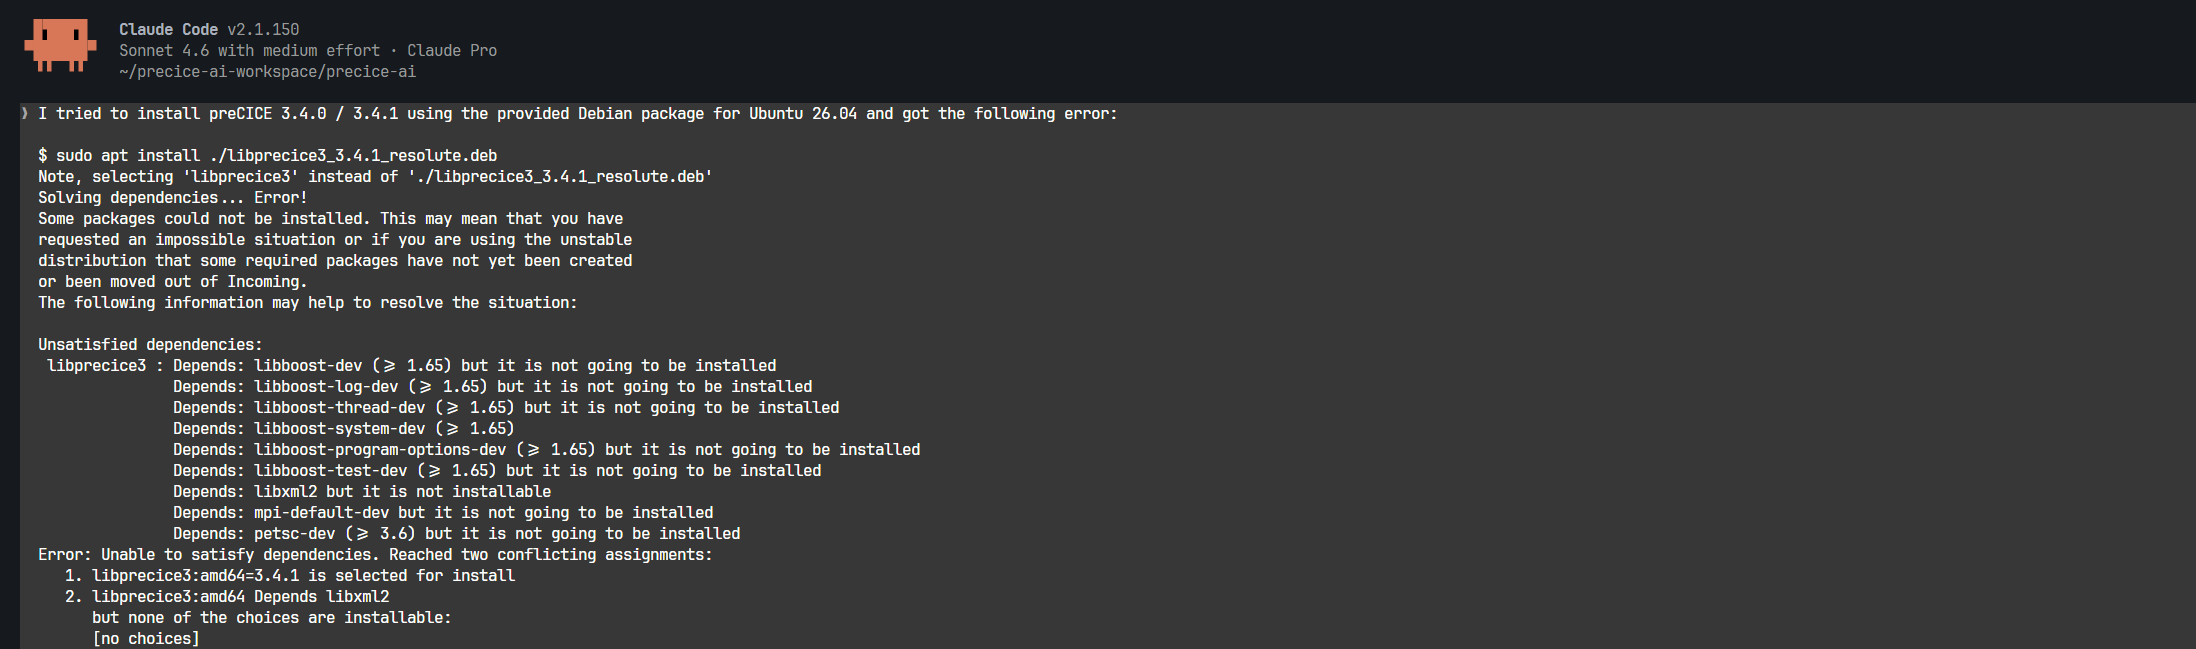
\includegraphics[width=1\linewidth]{precice-ai_issue_question}
  \caption{MCP server in action, answering a configuration question inside an \gls{mcp} client.}
  \label{fig:precice-ai_issue_question.png}
\end{figure}

\begin{figure}[htbp]
  \centering
  \framebox[\linewidth]{\parbox{\linewidth}{\centering\vspace{5cm}%
  \textit{[Screenshot placeholder: Claude Code session invoking the preCICE AI MCP server on a
  representative configuration-authoring or log-analysis task, showing the tool-call sequence
  and the resulting natural-language answer.]}%
  \vspace{5cm}}}
  \caption{Representative Claude Code session using the preCICE \gls{mcp} server on an
           evaluation scenario.}
  \label{fig:claude-code-screenshot}
\end{figure}

\begin{figure}[htbp]
  \centering
  \framebox[\linewidth]{\parbox{\linewidth}{\centering\vspace{5cm}%
  \textit{[Screenshot placeholder: Codex session invoking the preCICE AI MCP server on the same
  representative task as \cref{fig:claude-code-screenshot}, for direct visual comparison across
  MCP clients.]}%
  \vspace{5cm}}}
  \caption{Representative Codex session using the preCICE \gls{mcp} server on the same
           evaluation scenario.}
  \label{fig:codex-screenshot}
\end{figure}

\begin{figure}[htbp]
  \centering
  \framebox[\linewidth]{\parbox{\linewidth}{\centering\vspace{4cm}%
  \textit{[Planned figure: grouped bar chart showing task completion accuracy (cosine
  similarity for easy-tier questions; qualitative rating converted to a numeric scale for
  medium- and difficult-tier questions) per scenario category, broken down by prototype
  (MCP server, LangGraph agent, baseline), knowledge-base retrieval mode (lexical, semantic),
  and model tier (small, mid-tier, frontier). To be completed when evaluation runs are
  finished.]}%
  \vspace{4cm}}}
  \caption{Planned task completion accuracy across prototypes, retrieval modes, model tiers,
           and difficulty tiers.}
  \label{fig:accuracy-grid}
\end{figure}


% ----------------------------------------------------------------
\section{Discussion (SM6)}\label{sec:evaluation:discussion}
% ----------------------------------------------------------------

\emph{Full interpretation will follow the completion of the evaluation runs described in
\cref{sec:evaluation:setup,sec:evaluation:execution}.}

The preliminary retrieval results (Precision@5 of 0.82) indicate that semantic search over the
preCICE documentation category is already accurate enough to provide useful grounding for the
majority of user queries.
The lower precision observed for coupling-scheme tuning queries (0.72) likely reflects the fact
that tuning advice is distributed across multiple documentation sections and forum threads,
making it harder to retrieve in a single top-5 set; the planned lexical-versus-semantic
comparison, and the forum and issue-tracker categories that the preliminary evaluation did not
yet cover, are both expected to shed further light on this category specifically.

Functional testing confirms that the \gls{mcp} server is robust to malformed inputs and handles
error cases gracefully across all five tool groups, including the \gls{cli}-wrapper group added
after the initial three-group design.
The plain-text tool output format was found to be well-suited for \gls{llm} consumption, with
concise, purpose-built summaries enabling the model to reference specific facts in its responses
rather than restating entire file contents.

The qualitative comparison in \cref{tab:approach-comparison} suggests that the \gls{mcp} server
prototype offers broader client compatibility and a more reproducible knowledge base, while the
LangGraph prototype offers a continuously refreshed retrieval index and full ownership of the
orchestration loop, at the cost of a heavier local footprint.
The full evaluation, once executed across the knowledge-base, model-tier, and difficulty grid
defined in \cref{sec:evaluation:setup}, is expected to clarify two open questions in particular:
whether the accuracy advantage of grounding is concentrated in the weaker model tier, as
hypothesized, and whether semantic retrieval meaningfully outperforms the network-independent
lexical path once evaluated beyond the single preliminary query sample reported above.


%%% ===============================================================
\chapter{Conclusion and Outlook}\label{sec:conclusion}
%%% ===============================================================

This thesis presents preCICE AI, a context-aware intelligent assistant for the preCICE
multi-physics coupling library.
The work is motivated by the significant usability gap between the capabilities of modern
\glspl{llm} and the practical needs of preCICE users---a gap that arises not from insufficient
model intelligence, but from the absence of grounded access to local project state and
domain-specific knowledge.

\paragraph{Contributions.}
The completed contributions of this work are:

\begin{enumerate}
  \item A systematic analysis of the preCICE user workflow identifying the information sources
        and operations required by an intelligent assistant (\cref{sec:problem-exposition}).
  \item The design and implementation of a preCICE \gls{mcp} server with five tool groups,
        26 tools in total, covering project discovery, configuration inspection, log analysis,
        knowledge-base retrieval, and a wrapper around the official preCICE \gls{cli}
        (\cref{sec:mcp-server}).
  \item The design and implementation of a dual lexical-and-semantic retrieval pipeline over
        seven categories of preCICE knowledge, including documentation, tutorials, the
        Discourse forum, and the GitHub issue tracker, published through versioned release
        assets and validated by a preliminary retrieval-quality assessment
        (\cref{sec:context-retrieval}).
  \item A second, architecturally independent prototype built with LangGraph that reuses the
        same class of tools inside a self-contained ReAct agent and its own browser interface,
        and that can in turn drive the \gls{mcp} server as a subprocess
        (\cref{sec:claudecode-approach}).
  \item An evaluation design spanning both prototypes, two knowledge-base retrieval modes,
        three language-model capability tiers, and three question-difficulty tiers, combining
        automated similarity-based scoring with manual qualitative assessment
        (\cref{sec:evaluation}).
\end{enumerate}

\paragraph{Answers to research questions.}
RQ1 (Tool integration) has been addressed by the implemented \gls{mcp} server, which
demonstrates that the five identified tool groups are sufficient to support project overview,
configuration inspection, log analysis, knowledge retrieval, and \gls{cli}-backed validation
tasks across a set of representative preCICE projects.
RQ2 (Context retrieval) is substantially addressed: both the lexical and semantic retrieval
paths have been implemented over the full seven-category knowledge base, and a preliminary
quality assessment of the semantic path shows encouraging results, while the systematic
comparison between the two paths across model tiers and difficulty levels remains to be
executed.
RQ3 (Prototype comparison) will be fully addressed by the evaluation runs described in
\cref{sec:evaluation}, which are planned but not yet executed at the time of writing.

\paragraph{Limitations.}
The current prototypes have several limitations.
First, the full evaluation across knowledge-base modes, model tiers, and difficulty levels has
not yet been executed, so the quantitative claim that preCICE AI improves task completion over
an ungrounded baseline, and the claim that grounding matters more for weaker models, both remain
to be validated rather than assumed.
Second, the \gls{mcp} server's configuration tools remain deliberately conservative: they
inspect, summarize, and back up the configuration file, but do not yet apply edits directly,
leaving configuration-authoring tasks as a suggest-and-copy workflow for the user rather than a
suggest-and-apply one.
Third, the two prototypes' retrieval pipelines have not been benchmarked against each other
directly, only against a shared baseline, which limits how confidently the qualitative
comparison in \cref{tab:approach-comparison} can be read as a ranking rather than as a
description of two different design points.
Fourth, the LangGraph prototype's own knowledge-base ingestion pipeline still depends on
components, such as a local vector-database client and embedding library, that were introduced
during an earlier design iteration and are no longer exercised by every code path, which is a
maintainability concern more than a correctness one but is worth resolving before further
extension.

\paragraph{Future work.}
Several directions for future work are motivated by the analysis and preliminary results:

\begin{itemize}
  \item \emph{Write-capable configuration tools:} Extending the configuration tool group with
        carefully scoped write operations, building on the existing backup tool, would enable
        the assistant to apply suggested changes directly rather than presenting them as text
        for the user to copy.
  \item \emph{Direct retrieval-pipeline comparison:} Running the same question set through both
        prototypes' retrieval pipelines under matched conditions would clarify whether a
        pre-built, periodically republished knowledge base or a continuously self-refreshing
        one is the better default for a locally run assistant.
  \item \emph{Simulation execution tools:} A tool that can launch and monitor a preCICE
        simulation would support the full phase-3 workflow, which today still requires the user
        to start the simulation outside the assistant.
  \item \emph{Broader evaluation:} A user study with preCICE practitioners would provide
        ecologically valid evidence of the assistant's utility beyond the controlled,
        scenario-based evaluation designed in this thesis.
  \item \emph{Security hardening beyond the current allowlist:} As the tool surface grows,
        periodically revisiting the command-execution allowlist and blocklist against the kind
        of \gls{mcp}-specific threat models identified by \citeauthor{hou2025mcplandscape}
        \cite{hou2025mcplandscape} and the benchmarked attack patterns of
        \citeauthor{wang2025mcptox} \cite{wang2025mcptox} would help keep the safety posture
        proportionate to the capability being added.
  \item \emph{Generalization to other coupling libraries:} The \gls{mcp} server architecture
        and retrieval pipeline design are not specific to preCICE and could be adapted to other
        scientific simulation frameworks with relatively modest effort.
\end{itemize}

preCICE AI demonstrates that standards-based tool integration via \gls{mcp}, combined with
domain-specific \gls{rag} and, where useful, a self-contained agent runtime built directly on
the same tools, is a viable architecture for making complex scientific simulation software more
accessible to users of all experience levels.


%%% ===============================================================
%%% Bibliography
%%% ===============================================================

\printbibliography

\ \\
\noindent
All links were last followed on May 20, 2026.

\clearpage
\appendix
\addcontentsline{toc}{part}{Appendix}

%%% ===============================================================
\chapter{MCP Server Tool Reference}\label{sec:appendix-tools}
%%% ===============================================================

This appendix provides a complete reference for all 26 tools implemented in the preCICE
\gls{mcp} server, grouped as in \cref{sec:mcp-server}.

\section{Project Tools}

\begin{description}[font=\ttfamily]
  \item[list\_precice\_projects]\mbox{}\\
        Lists the subdirectories of the configured projects root as candidate preCICE
        projects.\\
        \textit{Input:} none.\\
        \textit{Output:} plain-text list of project names.

  \item[inspect\_project\_structure]\mbox{}\\
        Returns a depth-limited directory tree for a named project.\\
        \textit{Input:} \texttt{project\_name} (string); \texttt{max\_depth} (integer,
        default 3).\\
        \textit{Output:} plain-text directory tree.

  \item[find\_precice\_config]\mbox{}\\
        Locates the \texttt{precice-config.xml} file within a named project.\\
        \textit{Input:} \texttt{project\_name} (string).\\
        \textit{Output:} the resolved configuration file path, or a not-found message.

  \item[run\_command\_in\_project]\mbox{}\\
        Executes an allowlisted, read-oriented shell command with a named project as its
        working directory.\\
        \textit{Input:} \texttt{project\_name} (string); \texttt{command} (string).\\
        \textit{Output:} captured standard output, standard error, and return code, or a
        refusal message if the command fails the safety check.
\end{description}

\section{Configuration Tools}

\begin{description}[font=\ttfamily]
  \item[inspect\_precice\_config]\mbox{}\\
        Reads and returns the structured contents of a project's configuration file.\\
        \textit{Input:} \texttt{project\_name} (string).\\
        \textit{Output:} plain-text structured description of participants, meshes, data
        fields, and the coupling scheme.

  \item[summarize\_precice\_config]\mbox{}\\
        Produces a concise, human-readable summary of the configuration file.\\
        \textit{Input:} \texttt{project\_name} (string).\\
        \textit{Output:} short plain-text summary.

  \item[backup\_precice\_config]\mbox{}\\
        Writes a timestamped copy of the current configuration file.\\
        \textit{Input:} \texttt{project\_name} (string).\\
        \textit{Output:} path to the created backup file.
\end{description}

\section{Log Tools}

\begin{description}[font=\ttfamily]
  \item[list\_project\_logs]\mbox{}\\
        Scans a named project for preCICE log files.\\
        \textit{Input:} \texttt{project\_name} (string).\\
        \textit{Output:} plain-text inventory of discovered log files.

  \item[read\_project\_logs]\mbox{}\\
        Reads the content of every discovered log file, truncated per file.\\
        \textit{Input:} \texttt{project\_name} (string); \texttt{max\_chars\_per\_file}
        (integer, default 5000).\\
        \textit{Output:} concatenated, truncated log contents.

  \item[read\_latest\_log]\mbox{}\\
        Reads the tail of the most recently modified log file.\\
        \textit{Input:} \texttt{project\_name} (string); \texttt{lines} (integer, default 80).\\
        \textit{Output:} the requested number of trailing lines.

  \item[analyze\_precice\_logs]\mbox{}\\
        Scans all log files for heuristic error, warning, and convergence indicator terms.\\
        \textit{Input:} \texttt{project\_name} (string).\\
        \textit{Output:} matched lines together with trailing log context.
\end{description}

\section{Knowledge Base Tools}

\begin{description}[font=\ttfamily]
  \item[kb\_precice\_status]\mbox{}\\
        Reports, per category, whether local knowledge-base assets are present and fresh.\\
        \textit{Input:} none.\\
        \textit{Output:} plain-text freshness report across all seven categories.

  \item[kb\_query\_precice]\mbox{}\\
        Answers a natural-language query against the locally cached semantic index for a given
        category.\\
        \textit{Input:} \texttt{query} (string); \texttt{category} (string).\\
        \textit{Output:} top-$k$ retrieved chunks with source metadata.

  \item[kb\_query\_precice\_live]\mbox{}\\
        As \texttt{kb\_query\_precice}, refreshing missing or stale category assets first.\\
        \textit{Input:} \texttt{query} (string); \texttt{category} (string).\\
        \textit{Output:} top-$k$ retrieved chunks with source metadata.

  \item[kb\_query\_precice\_lexical]\mbox{}\\
        Performs keyword-based retrieval against the lexical index; makes no external call.\\
        \textit{Input:} \texttt{query} (string); \texttt{category} (string, optional).\\
        \textit{Output:} top-$k$ retrieved chunks with source metadata.

  \item[kb\_ingest\_precice\_data]\mbox{}\\
        Triggers a local rebuild or refresh of knowledge-base assets.\\
        \textit{Input:} \texttt{category} (string, optional).\\
        \textit{Output:} status report of the ingestion run.
\end{description}

\section{CLI-Backed Tools}

\begin{description}[font=\ttfamily]
  \item[precice\_version]\mbox{}\\ Reports the installed preCICE \gls{cli} version.
  \item[precice\_config\_check]\mbox{}\\ Validates a configuration file via the reference
        \gls{cli}.
  \item[precice\_config\_visualize]\mbox{}\\ Produces a visual representation of the coupling
        topology.
  \item[precice\_config\_format]\mbox{}\\ Normalizes the formatting of a configuration file.
  \item[precice\_config\_doc]\mbox{}\\ Looks up reference documentation for a configuration
        element.
  \item[precice\_init]\mbox{}\\ Validates a topology against a \gls{json} schema and scaffolds
        a new project.
  \item[precice\_profiling\_analyze]\mbox{}\\ Summarizes profiling output from a preCICE run.
\end{description}

Every tool in this group first checks for \texttt{precice-cli} on the system path and returns
an installation hint instead of failing when it is absent, as described in
\cref{sec:mcp-server:cli-tools}.


%%% ===============================================================
\chapter{Minimal preCICE Configuration Example}\label{sec:appendix-config}
%%% ===============================================================

\Cref{lst:minimal-config} shows the structure of a minimal \texttt{precice-config.xml} file
for a two-participant serial explicit coupling, illustrating the elements parsed by the
configuration tool group described in \cref{sec:mcp-server:config-tools}.

\begin{listing}[htbp]
\begin{minted}[linenos=true]{xml}
<?xml version="1.0" encoding="UTF-8" ?>
<precice-configuration>
  <log>
    <sink filter="%Severity% > debug" enabled="true"/>
  </log>
  <data:scalar name="Pressure"/>
  <data:vector name="Velocity"/>
  <mesh name="Fluid-Mesh" dimensions="3">
    <use-data name="Pressure"/>
    <use-data name="Velocity"/>
  </mesh>
  <participant name="Fluid">
    <provide-mesh name="Fluid-Mesh"/>
    <write-data name="Velocity" mesh="Fluid-Mesh"/>
    <read-data  name="Pressure" mesh="Fluid-Mesh"/>
  </participant>
  <m2n:sockets acceptor="Fluid" connector="Solid"/>
  <coupling-scheme:serial-explicit>
    <participants first="Fluid" second="Solid"/>
    <max-time-windows value="100"/>
    <time-window-size value="0.01"/>
    <exchange data="Velocity" mesh="Fluid-Mesh"
              from="Fluid" to="Solid"/>
  </coupling-scheme:serial-explicit>
</precice-configuration>
\end{minted}
\caption{Minimal preCICE configuration file for a two-participant serial explicit coupling.
         Field and participant names are illustrative.}
\label{lst:minimal-config}
\end{listing}

\pagestyle{empty}
\renewcommand*{\chapterpagestyle}{empty}
\Versicherung
\end{document}